 \documentclass{article} %A4
\usepackage[a4paper,left=1.9cm, right=2.1cm,top = 1.2cm,bottom=2.3cm]{geometry}
\usepackage[utf8]{inputenc}%Umlaute
\usepackage[ngerman]{babel} %Texttrennung
\usepackage{graphicx}	%Grafiken
\usepackage{amssymb}
\usepackage{amsmath}
\usepackage{url}
\usepackage{listings}
 \usepackage{color}
\usepackage{hyperref}

\usepackage[labelformat=empty]{caption}
\title{Zusammenfassung - Web 2.0}
\author{
	Andreas Ruscheinski,
	Marc  Meier,
	Christian D.
}

\begin{document}
\maketitle
\setcounter{tocdepth}{1}
\tableofcontents
\section{Definitionsversuche}
	\subsection{Social Media, Enterprise 2.0, Web 2.0}
	\begin{itemize}
	\item\glqq Social Media bezeichnen digitale Medien und Technologien (vgl. Social Software), die es Nutzern ermöglichen, sich untereinander auszutauschen und mediale Inhalte einzeln oder in Gemeinschaft zu erstellen.\grqq (Wikipedia)\\
	\item\glqq Enterprise 2.0 bezeichnet im engeren Sinn den Einsatz von sozialer Software zur Projektkoordination, zum Wissensmanagement und zur Innen- und Außenkommunikation in Unternehmen\grqq (Wikipedia)\\
	\item\glqq Web 2.0 ist ein Schlagwort, das für eine Reihe interaktiver und kollaborativer Elemente des Internets, speziell des World Wide Webs, verwendet wird. Dabei konsumiert der Nutzer nicht nur den Inhalt, er stellt als Prosument selbst Inhalt zur Verfügung.\grqq (Wikipedia)
	\item Neue Technologien werden als Enabler gesehen d.h. Technologie ist Grundlange für die Unterstützung im Business Umfeld
	\item Verschiedene Modelle für die Beschreibung von Social Media, Enterprise 2.0, Web 2.0:
		\begin{itemize}
			\item Social Media Honeycomb
			\item SLATES
			\item FLATNESSES
		\end{itemize}
	\end{itemize}
	\subsubsection{Social Media HoneyComb}
	\begin{center}
	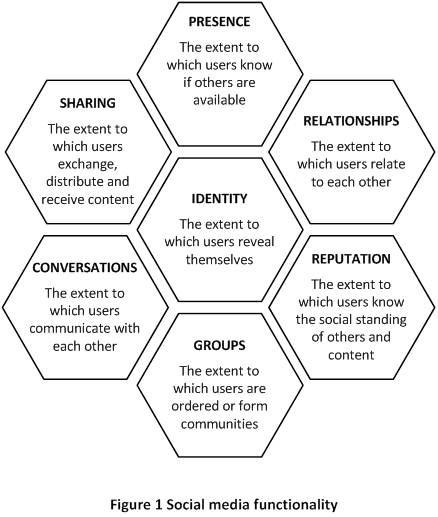
\includegraphics[scale=0.5]{img/SMHC_functionality.jpg}
	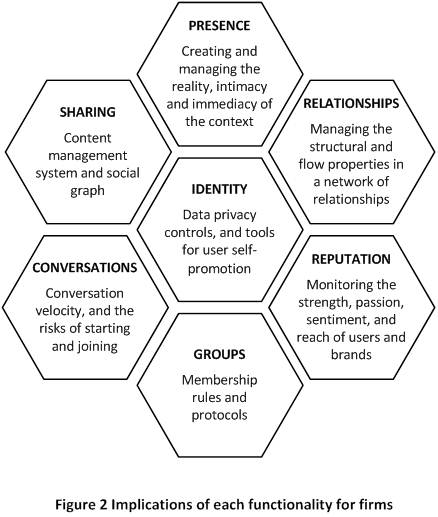
\includegraphics[scale=0.5]{img/SMHC_implications.jpg}
	\end{center}
	\begin{itemize}
		\item Charakterisierung möglich durch aus Wahl verschiedener Waaben als Baublöcke
		\item Hauptwaabe = Hauptaufgabe, Nebenwaaben = Zusätzliche Möglichkeiten
		\item  beschreibt, inwiefern sich Internetanwendungen durch das Ausmaß unterscheiden, in dem sie sich auf einige von sieben Social-Media-Bausteinen(Identität, Gespräche, Austausch, Präsenz, Beziehungen, Reputation und Gruppen) konzentrieren.
	\end{itemize}
	\subsubsection{SLATES}
	\glqq SLATES is an initialism that describes the business impacting capabilities, derived from the effective use of Web 2.0 technologies in and across enterprises.\grqq (Wikipedia), Jedes Element beschreibt eine zentrale Komponente von Enterprise 2.0
	\begin{description}
		\item[SEARCH] Unterstütze die unternehmensweite Suche nach Inhalten;
		Finden, was das Unternehmen weiß und in welchen Köpfen
		\item[LINKS] Ähnliches verbinden nach Assoziationen und Gemeinsamkeiten;
		Abkehr vom  \glqq Teile und herrsche\glqq 
		\item[AUTHORSHIP] Niedere Barrieren für Authorship;
		Jeder kann und soll sich als Autor kreativ einbringen
		\item[TAGS] Jeder kann dem Wissen seine Strukturen überstülpen;
		Emergente Strukturen lösen starre Hierarchien und Schemata ab
		\item[EXTENSIONS] Erweiterung der eigenen Sicht und Bewertung;
		Empfehlungssysteme, Bewertungsportale
		\item[SIGNALS] Push und Pull durch Signal-basierte Kanäle ersetzen
	\end{description}
	\subsubsection{FLATNESSES}
	FLATNESS ist eine Erweiterung für SLATES basierend auf der Beobachtung von Enterprise 2.0 in Aktion. Einige Beobachtungen:
	\begin{itemize}
		\item Enterprise 2.0 is going to happen in your organization whether you
		like it or not
		\item Enterprise 2.0 doesn’t seem to put older IT systems out of business
		\item the benefits of Enterprise 2.0 can be dramatic, but only build steadily
		over time
	\end{itemize}
	\begin{center}
		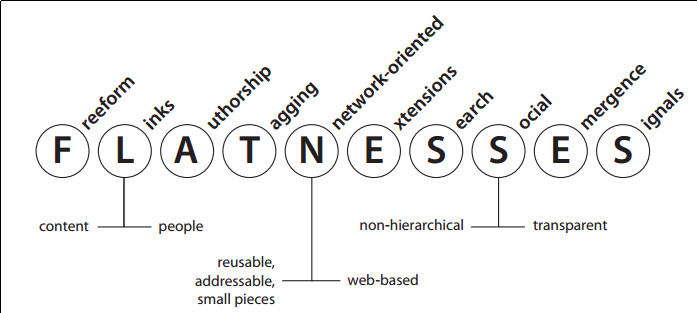
\includegraphics[scale=0.5]{img/FLATNESS.jpg}
	\end{center}
	\subsection{Vergleich Enterprise 1.0 und Enterprise 2.0}
	\begin{center}
		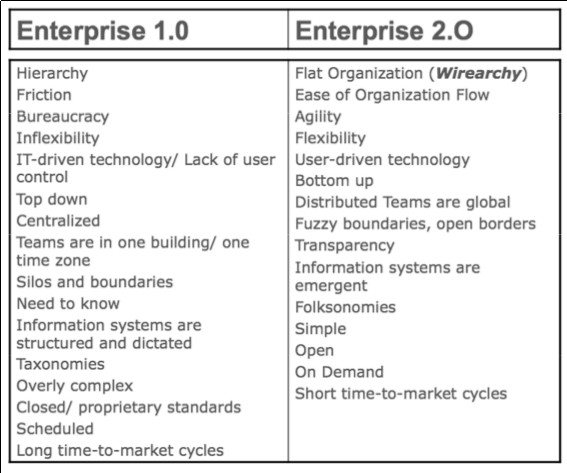
\includegraphics[scale=0.8]{img/CompareW1W2.jpg}
	\end{center}
	\subsection{Konzepte}
	\begin{itemize}
		\item Entwicklung des Web 2.0 führte zu einer Reihe neuer Ansätze
		\begin{description}
			\item[User Interface:] Lightweight Rich Client, Ajax, Desktop Feel
			\item[Content:] User Generated Content, Prosumer
			\item[Cooperation:] Wisdom of Crowd, Crowd Sourcing
			\item[Economy:] Attention, Intention, Network Economy
			\item[Life Cycle:] Perpetual Beta, Consumer designed product
			\item[Social Media:] facebook usw...
		\end{description}
		\item zentrale Merkmale: Interaktion, Kollaboarion, Sharing, User Generated Content
	\end{itemize}
	\subsubsection{Anwendungen - User Generated Content}
	Der Inhalt wird durch den User erstellt. Mögliche Kategorisierung von Web 2.0 Anwendungen:
		\begin{description}
			\item [Upload Content:] Der Benutzer lädt den Inhalt einer Webseite hoch, Bsp: Youtube, Flickr
			\item [Complete User Dominance:] Der Benutzer ist zentrales Element der Webseite, Bsp: Foren, Blogs, Wikis, Twitter
			\item [Trust Themen:] Wie vertrauenswürdig ist der erstellte Content? 
			\item [Kollaboration:] Die Benutzer arbeiten Zusammen, Bsp: Google Docs, Etherpad $\rightarrow$ Prosumers
		\end{description}
	\subsubsection{Anwendungen - Cooperation Portals}
	 Mögliche Kategorisierung von Coopartion Portale:
		\begin{description}
			\item[Business Networks:] Plattform für den Austausch von unternehmesrelevanten Informationen, Bsp: XING; LinkedIn
			\item[Interest Networks:] Plattform für den Austausch von Interessen der Benutzer, Bsp: Facebook, MySpace
			\item[Synchronisation:] Plattform für die Synchronisation von Benutzerinformationen über verschiedene Endgeräte, Bsp: Foxmarks(Lesezeichen), Plaxo(Kontaktdaten)
		\end{description}
	\subsubsection{Technologien - Konzepte}
	\begin{description}
		\item[Advanced JavaScript:] Einsatz von komlexen JavaScript Programmen für die Realisierung der Webseite
		\item[AJAX, XHR, HTML5:]  Realisierung einer dynamischen Webseite durch asynchrone Kommunikation
		\item[Folkonomies und Tags:] Webseite stellt eine Benutzer definierte Möglichkeit für die Organisation der Daten, Bsp: Hashtag, Subreddit
		\item[Browser Extensions und Plugins:] Erweiterung der Browser durch den Anwendungsentwickler, dadurch Desktop Look-and-Feel
		\item[Probabilistische Algortihmen (Bitcoin):] Einsatz von Probablistischen Algorithmen auf verteilter Basis für die Erbrining einer Leistung, Bsp: Bitcoin(Online Wallet)
	\end{description}	
	\subsubsection{Technologien - Werkzeuge}
	\begin{description}
		\item[JS Libraries:] jQuery, extJS, Angular
		\item[Embedded JS:] Einsatz von JavaScript auf Server/Desktop Ebene, Bsp: V8, node.js
		\item[Ajax KITS:] Implementierung für die asynchrone Kommunikation, Bsp: Rico, Dojo, GWT
	\end{description}
	\subsection{Notizen}
		\begin{itemize}
			\item Silos and Boundaries
				\begin{itemize}
					\item Problem bei nicht-Silos: Snowden $\rightarrow$ Daten werden selbstständig
					\item Silos sind alles an Daten, die in einem Umfeld formatiert sind, die man aber irgendwann nicht mehr interpretieren kann $\rightarrow$ sie werden inkompatibel
					\item Wünschenswert: Migration von bspw. Facebook zu MySpace
				\end{itemize}
				\item Prosumers: Nutzer in der Doppelrolle \glqq Inhalt von allen für alle\grqq
				\item Die Daten-Sammel-Phase ist zuende $\rightarrow$ wie sollen sie verarbeitet werden? $\rightarrow$ Google weiß bspw. schon vorher ob eine Grippewelle eintritt
		\end{itemize}
		
		
		
	\section{AJAX und Web 2.0}
	\subsection{Allgemein}
	\begin{itemize}
		\item AJAX ist KEINE neue Technologie sondern Design Pattern
		\item Problem: Verhalten des Benutzers anders als bei Desktop Anwendungen
		\begin{itemize}
			\item Blättern durch einzelne Seiten
			\item Wenig Interaktivität 
			\item Kein undo/redo
			\item Viele Unklarheiten - Reload, Bookmarks und zurück
		\end{itemize}
	\end{itemize}
	\subsection{Vergleich der Reload Cycles}
	\begin{center}
		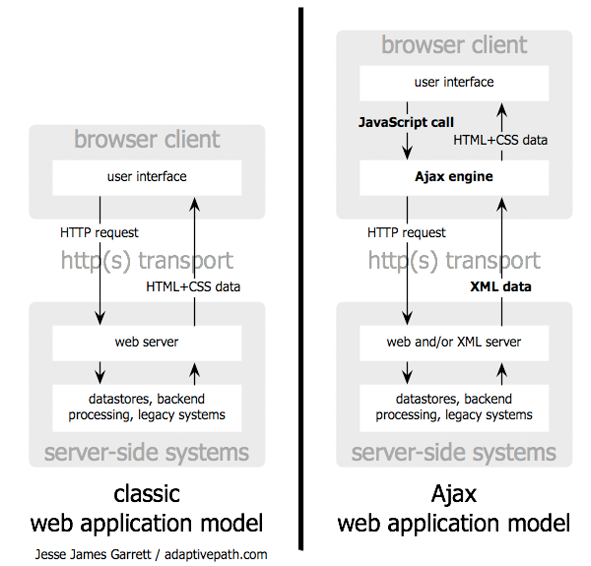
\includegraphics[scale=0.5]{img/HTTP_Ajax.png}
	\end{center}
	\subsection{AjaX}
	\begin{itemize}
		\item AjaX = Asynchronous JavaScript XMLHTTPRequest (XHR)
		\item Asynchron = GUI nicht blockiert während Übertragung
		\item kein neuer Seitenaufbau sondern dynamische Erweiterung mittels JavaScript
		\item Arbeitet als Single-Thread, was kritische Probleme löst (Es muss nicht auf parallele Entwicklung geachtet werden)
	\end{itemize}
	\subsection{Konzepte und Technologien}
	\begin{itemize}
		\item Schwächer gekoppelte Kommunikation
		\begin{itemize}
			\item Asynchrone Kommunikation: XMLHttpRequest, Sockets
			\item Varianten der synchrone Kommunikation: Multipart MIME, Server Sockets
		\end{itemize}
		\item Leichtgewichtiges Processing in n-tier Denkweise
		\begin{itemize}
			\item Client-Side Scripting: JavaScript
			\item Server-Side Code Generation: PHP, Java – basierte Ajax Kits
		\end{itemize}
		\item OO Dokumentenmodell mit Repräsentationsabtrennung
		\begin{itemize}
			\item Markup: HTML, XML, XHTML
			\item Repräsentations Transformation: CSS, XSLT
			\item DOM – Manipulation: innerHTML, JS DOM
		\end{itemize}
	\end{itemize}
	\subsection{First Player und Impulse}
	\begin{itemize}
		\item Es wird früh eine Entscheidung gefällt, sodass sich spätere und bessere Lösungen nicht mehr durchsetzen können. Aufkaufen der Konkurrenz sichert die eigene Existenz
		\item Google Suggest: Interactive GUI
		\item Writely $\rightarrow$ Google Docs
		\item Google Maps und Gmail
		\item Technorati (Realtime Trend Analyse mit humane Klassifikation)
		\item Flickr und Youtube (Prosument)
		\item The Broth (Multiuser Game (Mosaik),JS basiertes Drag-and-Drop)  
		\item LinkedIn
	\end{itemize}
	\subsection{Wirtschaftliche Aspekte}
	Einfach mal in den Folien lesen \glqq02-netzwerk-effekte-2015-bw.pdf\grqq
		\begin{itemize}
			\item Lizensierung\\
			(Office like oder Apps)
			\item Lock up in the Cloud\\
			(Amazon und Weihnachten)
			\item Lock up in the App
			\item Lock up in the App Store
			\item Half-Open Source\\
			(Pro open-Source: entwickelt für mich; Contra: gewisser Kontroll-Verlust)
			\item Affero Lizenz
			\item Mandatory Binary Signing
		\end{itemize}
		\subsection{Geschäftsprobleme im Internet}
			Das Problem:
			\begin{itemize}
				\item Viele (gute) Lösungen sind kostenfrei\\
				(warum was zahlen?)
				\item Metering ist schwierig\\
				(Wie messe/berechne ich Nutzung?)
				\item Brand Building ist extrem teuer (bspw. Apple/Google)
				\item Advertising ist ausgelutscht				
			\end{itemize}
			Die Kernfragen:
			\begin{itemize}
				\item Wer zahlt an wen?
					\begin{itemize}
						\item Oft nicht der unmittelbare Nutznießer der Dienstleistung
						\item Bsp: Google: Es zahlt nicht der Such-Kunde (Finanziert sich durch Aufmerksamkeits-Lenkung)
						\item Bsp: Firefox: Es zahlt nicht der Browser-Kunde (Finanziert sich durch Default Homepage / Search Engine Google)
					\end{itemize}
				\item Warum wird gezahlt? 
					\begin{itemize}
						\item Geleisteter Dienst, aber auch ausgenutzte Bindungen
						\item Bsp: Facebook: Kenntnis der Daten des Endanwenders
						\item Bsp: AppStore: Zwangsbündelung über Installation
					\end{itemize}
				\item Wofür wird gezahlt?
					\begin{itemize}
						\item Für Daten oder Dienste
						\item Für ein Enabling (Zugang, Default-Einstellung, Top Platzierung)
					\end{itemize}
				\item Wie schützt sich das Modell vor Nachahmung?
			\end{itemize}
		Mögliche Lösungen
			\begin{itemize}
				\item Premium Services sind kostenpflichtige high-end Versionen einer Dienstleistung
				\item Commercial Services sind Versionen einer Dienstleistung für den comm./prof. User\\
				(Zuverlässigkeit, Features, Rechtsgarantien)
				\item Technologie-Kompetenz als Outsourcing einer high-end IT Abteilung
				\item Solution Hosting betreibt eine komplexe Technologie Server-seitig
				\item Infomediary betreibt einen Handelsplatz zwischen Bedürfnissen
				\item Verbund-Angebote / Lock-In Angebote
			\end{itemize}
			
						
	\section{XMLHttpRequest}
	\begin{itemize}
		\item XMLHttpRequest ist ein JS Objekt, REQUEST öffnet HTTP Verbindung, RESPONSE verwaltet die Antwort
		\item Allgemeines Vorgehen:
		\begin{enumerate}
			\item Neues XMLHttpRequest-Objekt erstellen
			\item Request spezifizieren: TYP(GET,POST,PUT,DELETE,\dots),URL (ggf. mit Query Encoding), Boolean Asyc (True für Asynchrone Kommunikation, False für Synchrone Kommunikation)
			\item Setzen des Event Handlers (eine Funktion), welcher ausgeführt wird, wenn Antwort vom Server kommt
			\item Senden des Request ggf. mit Body (bei POST leer)
		\end{enumerate}
		\item GET ist relativ unsicher (leicht einsehbar, gilt nicht bei XHR), ggf. Problem mit Firewalls (Empfohlen wenn wenig Daten im Query)
		\item POSTS werden nicht gecached und nervige Browsermeldung (nicht bei XHR) (Empfohlen bei vielen Daten im Query)
		\item Synchron (nicht Ajax): sinnvoll wenn die Interaktion des Users zu verhinden (Bsp.: online Banking)
		\item Asynchron: Programieraufwand (Timeout, Fehlerfall, Mehrfach-Requests, Anzeige an die User über laufenden Ladevorgang)
		\item Umgang mit Fehlerfällen: Defensiv Programmieren: überall entsprechende Exception Handler vorsehen, Viel Logging, Davon ausgehen, dass alles irgendwann mal irgendwie schief läuft
	\end{itemize}
			
	
	\section{Netzwerk Effekte}	
	\subsection{Struktur und Wert}
	\begin{enumerate}
		\item Sarnoff \textbf{Content is King}
		\begin{itemize}
			\item \textbf{Nutzen}: Anzahl der Knoten
			\item \textbf{Entscheidung}: ob man das Angebot nutzt oder nicht
			\item \textbf{Wert}: Linear zur Netzwerk-Größe (n)
			\item \textbf{Bsp}: Radio-Sender
			\item \textbf{Wettbewerb}: Friedvolle Koexistenz, Größe $\rightarrow$ Fitness
			\item \textbf{Zusammenschluss}: Werte der Netze addieren sich bei Zusammenschluss ($n + m$)
			\item Best Content
		\end{itemize}
		\item Metcalfe \textbf{Transaction is King}
		\begin{itemize}
			\item \textbf{Nutzen}: Anzahl Verbindungen
			\item \textbf{Entscheidung}: welchen Peer kontaktiere ich?
			\item \textbf{Wert}: $n^2$ genauer: n*(n-1)/2
			\item \textbf{Bsp}: Telefon, E-Mail
			\item \textbf{Wettbewerb}: Survival of the Fittest (Darwin)
			\item \textbf{Zusammenschluss}: Der Wert ist mehr als die Addition der Werte der Ausgangsnetze ($n^2 + m^2 + 2nm$)
			\item Most Members
		\end{itemize}
		\item Reed \textbf{Cooperation is King}
		\begin{itemize}
			\item \textbf{Nutzen}: Anzahl Subgruppen
			\item \textbf{Entscheidung}: Welche Gruppen bilde ich?
			\item \textbf{Wert}: Exponentiell: $2^n$
			\item \textbf{Bsp}: Google +, Blogs, Wikis, Usenet, Facebook
			\item \textbf{Wettbewerb}: Theoretisch: One choice for ever (Eigen)
			\item \textbf{Zusammenschluss}: Die Werte multiplizieren sich.
			\item Best Facilitation
		\end{itemize}
	\end{enumerate}
	\begin{itemize}
		\item Benutzer-initiierte Interessengruppen fördern
		\item Maximales initiales Investment (sichert \glqq one choice for ever\grqq, aber maximales Risiko)
	\end{itemize}
	\subsection{Effekte und Strategien}
	\begin{itemize}
		\item Nutzen für den einzelnen Teilnehmer verändert sich
abhängig von der Zahl an Teilnehmern am Gesamtsystem
		\begin{description}
			\item[Positiv:] Je mehr Teilnehmer desto mehr Leute kann man ansprechen
			\item[Negativ:] Je mehr Teilnehmer desto mehr Aufwand beim Filtern von Spam
		\end{description}
		\item Direkte Netzwerk-Effekte
		\begin{itemize}
			\item Abhängig von der Größe der Gruppe des Nutzers im Netzwerk
			\item Wenn viele meiner Bekannten E-Mail nutzen, so erhöht sich mein eigener Nutzen
		\end{itemize}
		\item indirekte Netzwerk-Effekte
		\begin{itemize}
			\item Nebeneffekt der Tatsache, daß ein Netzwerk
insgesamt viele Mitglieder hat
			\item Wenn E-Mail von vielen Menschen genutzt wird, so erhöht
sich mein eigener Nutzen, weil sich damit Dienstqualität und
Preis/Leistungsverhältnis verbessern
		\end{itemize}
	\end{itemize}
	\subsection{Zweiseitige Märkte}
		\begin{itemize}
		\item Das wesentliche Merkmal zweiseitiger Märkte sind gegenseitige, indirekte Netzwerkeffekte. Auf zweiseitigen Märkten treffen (mindestens) zwei unterscheidbare Gruppen von Akteuren aufeinander, deren Nutzen an der Plattform steigt, wenn die jeweils andere Gruppe auf der Plattform größer wird.
		
Nehmen wir das Beispiel von eben noch einmal auf: Betriebssysteme wie Windows sind zweiseitige Märkte. Warum: Weil, wie eben beschrieben, die Attraktivität des Betriebssystems für den Endnutzer (Gruppe A) steigt, wenn viele Programme dafür zur Verfügung stehen. Gleichzeitig steigt die Attraktivät des Betriebssystems für die Entwickler (Gruppe B), wenn es von sehr vielen Endnutzern (Gruppe A) und damit potentiellen Kunden eingesetzt wird.\\
\url{http://www.neunetz.com/2010/04/02/zweiseitige-maerkte-die-grundlagen/}
			\item Märkte, die zwei/mehrere unterschiedliche Teilnehmergruppen zusammenführen
			\item \glqq \textbf{Henne-Ei-Problem}\grqq
			\begin{itemize}
				\item First-Mover-Problem
				\item Förderung (Lösung und Problem), da es den Weg für Second-Mover bereitet				
			\end{itemize}
			\item Subvention
				\begin{itemize}
					\item Gruppe, die mehr von Netzwerk-Effekten zu profitieren glaubt unterstützt die anderen Gruppen
					\item bspw. durch Subventionen (Smartphone, Playstation)
				\end{itemize}
			\item Dominanz der Netzwerk-Effekte\\
			(Ein System, das größer ist als die Konkurrenz, bietet aufgrund direkter
Netzwerk-Effekte mehr Nutzen als ein kleineres, besseres System)
			\item Monopol-Situation\\
			(Einstiegshürden für Konkurrenz zu hoch)
			\item Lock-In-Effekt\\
			(Wechsel auf Konkurrenz-System ist teuer)
			\item Pinguin Effekt
				\begin{itemize}
					\item Früher Nutzer zieht keinen Nutzen aus einem Netzwerk da noch wenige andere Nutzer beteiligt sind
					\item \textbf{Negativer Fall}: Idee geht pleite bevor sie User hat
					\item \textbf{Positiver Fall}: Alle springen rein, sobald es läuft
				\end{itemize}
			\item \textbf{First Mover Strategien}
				\begin{itemize}
					\item Henne-Ei-Problem und hohe Initialkosten
					\item Konzept bekannt machen und weiterentwickeln
					\item Bindungschancen sichern initiales Investment 
					\item Zielgruppe: Early Adopters
				\end{itemize}
			\item \textbf{Second Mover Strategien}
				\begin{itemize}
					\item Typischerweise: Microsoft (plötzlich gibt es etwas und Microsoft taucht auf)
					\item Keine hohen Initialkosten
					\item Nutzt ausgereifte Konzepte
					\item Risiko: kann nicht mehr schnell genug in den Markt wachsen
				\end{itemize}
			\item \textbf{Kosten der Bekanntmachung}
			\begin{itemize}
				\item Virale Verbreitungstechniken\\
				(Nutzer als Konzept-Verbreiter und in möglichst vielen Teilnehmergruppen sein)
				\item Subventionieren einzelner Teilnehmergruppen\\
				(bspw Handy - dafür teure Verträge und Apps)
				\item Hypen + Pushen + Herumgeheimniseln (Apple)
			\end{itemize}
			\item \textbf{Kosten der Weiter-Entwicklung}
			\begin{itemize}
				\item Open / Crowd Sourcing
				\begin{itemize}
					\item Crowd-Sourcing der Reifungs-Kosten: Community development
					\item Crowd-Sourcing der Wartungs-Kosten: Community bug fixes
					\item Gefahr: Übernahme des Projekts durch andere \& Nachahmung
				\end{itemize}
				\item Plug In Architekturen\\
				(Konzept-Weiterentwicklung ohne die Grundidee zu kompromittieren)
				\item Virales Copyright (Jeder darf weiterentwickeln)
				\begin{itemize}
					\item Klassisch: Derivate unterstehen derselben Lizenz
					\item Dual Licensing: Kommerzielle Nutzung der Derivate Dritter erfordert Lizenz
				\end{itemize}
			\end{itemize}
			\item \textbf{Initiale Bindungschancen} (Dem Second Mover den Einstieg erschweren)
			\begin{itemize}
				\item Intellectual Property Protection
				\begin{itemize}
					\item Patent: Konzept kann nicht übernommen werden
					\item Copyright: Implementierung kann nicht übernommen werden
					\item Problem: In Konflikt mit Crowd Sourcing Konzept
				\end{itemize}
				\item User LockIn
				\begin{itemize}
					\item Benutzer kennt meine \textbf{GUI} \& \textbf{Konzepte} $\rightarrow$ Will nicht wechseln da gewohnt \& erlernt
					\item \textbf{Investment}: Benutzer hat Zeit in mein System investiert Upload von Profil + Inhalt, \\
					personalisiert, Akzeptieren von Freundschaften, Bewerten von Objekten, Erreichen von Status
				\end{itemize}
			\end{itemize}
			\item \textbf{Vorhandene Bindungschancen} (Dem First Mover die Entwicklung erschweren)			
			\begin{itemize}
				\item Nutze Chancen zur Bindung, die bereits bestehen
				\item Positionierung \glqq nur\grqq als Feature bekannter Konzepte
				\item Enge Integration in bestehendes Produkte
			\end{itemize}
			\item Zielgruppe
			\begin{itemize}
				\item \textbf{Early Adopters} kennen den letzten Schrei \& müssen ihn haben\\
				(Darf \& soll technisch, kompliziert \& Beta-Stadium sein und formen durch Feedback das Produkt weiter $\rightarrow$ Bsp: Linux)
				\item \textbf{Followers} folgen den Bewegungen der Masse\\
(Darf nicht den Touch des Technologischen haben; Übernehmen Produkt wie es ist;\\
hohe Erwartung an Stabilität; muss ausgereifte, standardisierte GUI \& Konzepte haben \\
$\rightarrow$ Bsp: Microsoft)
				\item \textbf{Kombination} oft versucht, nicht immer möglich (Bsp: Apple + Google)
			\end{itemize}
			\item Multihoming
			\begin{itemize}
				\item Mitglieder einer Gruppe eines mehrseitigen Markts auf mehreren Plattformen
				\item Mitglieder einer Gruppe findet man also auf mehr als einer Plattform wieder. Das erlaubt der anderen Gruppe einen größeren Spielraum bei der Wahl der jeweiligen Plattform.
				\item Bspw. Softwareentwickler, der für Windows und Mac entwickelt \& Geschäft, das mehrere Kreditkarten akzeptiert
				\item Multihoming wird notwendig, wenn konkurrierende Plattformen inkompatibel sind, aber Nutzen aus ihnen gezogen werden kann. Sofern mehrere konkurrierende Plattformen auf dem Markt sind, ist es nicht ungewöhnlich, dass mindestens eine Seite Multihoming betreibt.

\url{http://www.neunetz.com/2010/04/08/wie-multihoming-zweiseitige-maerkte-beeinflusst/}
			\end{itemize}
		\end{itemize}
	\subsection{Entwicklung am Beispiel der Browser Wars}
		\subsubsection{Netscape Mozilla Firefox}
		\begin{itemize}
			\item Nutzt erst \textbf{First} Mover Advantage
			\begin{itemize}
				\item Send Link… verbreitet Konzept der Webseiten per E-Mail
				\item View source… verbreitet Kenntnisse zur Entwicklung von Web-Seiten durch offenen Einblick in die Design-Dokumente für alle (Gegenbsp: Flash, PDF)
			\end{itemize}
			\item Nutzt dann \textbf{Second} Mover Advantage
			\begin{itemize}
				\item \textbf{Sicherer + stabiler} neue Angriffsposition, nutzt Crowd Sourcing Effekte bei der Behebung von Bugs
				\item \textbf{Auto-Update} bindet an vorhandene User Gemeinde
				\item \textbf{Fokus auf Follower} durch neue Positionierung: Gute GUI; vgl Thunderbird
"Reclaim your Inbox"
			\end{itemize}
		\end{itemize}
		\subsubsection{Microsoft Internet Explorer IE}
		\begin{itemize}
			\item Microsoft nutzt sehr oft Second Mover Advantage durch vorhandene Bindungschancen:
			\item Auslieferung des IE mit dem OS (Windows kommt mit IE installiert)
			\item Enge Integration des IE in das OS (Windows ohne IE funktioniert nicht
			\item IE übernimmt Rolle des Windows Exploreres
			\item IE kann mehr dank ActiveX
			\item \textbf{Problem beim Browser}: Unterschätzen der Second Mover Advantage von FFox
		\end{itemize}
		\subsubsection{Google Chrome}
		\begin{itemize}
			\item Mehr schon third move advantage !
			\item \textbf{Vorhandene Bindungschancen}:
			\begin{itemize}
				\item Besondere Search Features für Google Web Plattform (Search, Mail, Maps, Cal)
				\item Zuerst nicht unmittelbar ersichtlich (Bei Firefox durch PlugIns auch gegeben) $\rightarrow$ Besonders enge Integration mit Android Plattform macht wieder Sinn
			\end{itemize}
			\item \textbf{Google Strategie} (Search, Mail, Maps, Cal)\\
				$\rightarrow$ Verschenke wertvolles Produkt, um daüber woanders (Ads) Bindung zu erzielen
				\item \textbf{Android Strategie}\\
				$\rightarrow$ Schaffe Produkt, das per se Wert hat, um darüber woanders Bindung zu erzielen
		\end{itemize}
		
		
	\section{Bitcoin}
	\begin{itemize}
		\item \glqq Geld ist ein \textbf{Recht} zur Ausführung einer bestimmten Transaktion das von seinem \textbf{Träger} \textbf{genau einmal ausgeübt} werden kann und \textbf{nur durch} die Ausübung auf \textbf{andere übergeht}.\grqq
		\item Geld als Wertmaßstab, Tauschmittel und Wertaufbewahrung
		\item Bedrohungen: Wert-Verlust, Inflation, System-Crash,...
		\item \glqq Träger:\grqq
		\begin{itemize}
			\item an Name gebunden
			\item an Kenntnis gebunden
			\item an Pseudonym gebunden
			\item an den Besitz eines Objekts gebunden
			\item an Körper gebunden
		\end{itemize}
		\item \glqq Genau einmal ... von seinem Träger \grqq
		\begin{itemize}
			\item Geld kann nicht mehrfach ausgegeben werden
			\item Weitergabe möglich
			\item Backup nicht möglich
		\end{itemize}
		\item \glqq Nur durch\grqq
		\begin{itemize}
			\item Keine Erzeugung des Geldes ohne Deckung
			\item Gegenleistung in Zeit, Energie, Gold (Wert-Deckung)
			\item Gesellschaftlich Befugnis (Regelungs-Deckung)
			\item Gesellschaftliche Akzeptanz (De Facto Deckung)
		\end{itemize}
		\item \glqq auf andere übergeht\grqq
		\begin{itemize}
			\item einer verliert, einer bekommt das Recht
		\end{itemize}
		\item Wie entsteht der \glqq Wert\grqq des Geldes
		\begin{itemize}
			\item Geld lässt sich \textbf{unmittelbar konvertieren} in Nahrungsmittel, etc.
			\item Es wird akzeptiert und ist vom Gesetzt als Zahlungsmittel vorgeschrieben 
		\end{itemize}
	\end{itemize}
	\subsection{Was ist Bitcoin?}
	\begin{itemize}
		\item Träger des Geldes
		\begin{itemize}
			\item Bindung an Pseudonym (Bitcoin Adresse)
			\item Nachweis der Befugnis durch Schlüssel Paar
			\item Bitcoin Adresse ist Hashwert des public keys
			\item Private Key verlieren ist gleichbedeutend mit Geld verlieren
			\item Identität durch Schlüssel Paar Generierung (256 Bit)
		\end{itemize}
		\item Übertragung
		\begin{itemize}
			\item Peer-to-Peer
			\item Jeder Teilnehmer betreibt Bitcoin Knoten
			\item Jeder Knoten speichert Konto-Stände aller Adressen
			\item Transaktionen werden an alle Knoten gesandt
			\item Berechtigung wird durch Signatur überprüft
			\item Neue Kontostände werden an alle Knoten gesandt
		\end{itemize}
		\item Problem: Inkonsistente Kontostände (einige Knoten sind noch nicht über neue Kontostände informiert)
		\item Lösung: Bitcoin Blockketten-Algorithmus
		\item Wichtigste Aspekte von Bitcoin (hypeunabhänig)
			\begin{itemize}
				\item Hochreplizierte Datenbank
				\item Wird nach gewisser Zeit global konsistent
				\item probabilistischer Konsistenz-Begriff
			\end{itemize}
	\end{itemize}
	\subsection{Blockketten-Algorithmus}
	\subsection{Der ökonomische Ansporn}
		\begin{itemize}
			\item Warum sollten Leute Blöcke versiegeln wollen?
			\begin{itemize}
				\item Wer einen Block versiegelt, erhält 50 BTC
				\item Alle 4 Jahre wird der Wert halbiert $\rightarrow$ Asymptotisch: Maximal 21 Millionen BTC hergestellt\\				
				$\rightarrow$ Eingebauter Inflations-Schutz
				\item Algorithmus sieht vor: Überweisung wird nur durchgeführt, wenn eine kleine Fee\footnote{Bei dem dritten Wunsch weint | die gute Fee, weil es nicht bei den ersten zwei Löchern bleibt. | \glqq Es tut so weh\grqq} gezahlt wird
			\end{itemize}
			\item Konsequenzen
			\begin{itemize}
				\item Wird das Versiegeln ökonomisch unattraktiv
				\item[$\rightarrow$] dann versiegeln weniger Leute
				\item[$\rightarrow$] dann sinkt die Difficulty
				\item[$\rightarrow$] das Versiegeln kostet weniger CPU
				\item[$\rightarrow$] und wird dadurch wieder billiger
				\item[$\rightarrow$]\textbf{Stabiles, sich selbst regelndes System}
			\end{itemize}
			\end{itemize}
			
	\subsection{Problem: CAP-Theorem}
			\begin{itemize}
			\item Das Theorem
			\begin{enumerate}
				\item \textbf{C}onsistency: Alle Knoten sehen selbe Daten
				\item \textbf{A}vailability: System bleibt verfügbar bei einzelnen Knoten-Ausfällen
				\item \textbf{P}artition Tolerance: Netz-Partition macht kein Anhalten des Algorithmus erforderlich				
			\end{enumerate}
			\begin{itemize}
				\item In einem verteilten System bekommt man von CAP maximal 2 Eigenschaften hin $\rightarrow$ Bewiesen 2002
				\item Bitcoin garantiert alle 3 \\
				(C aber nur im probabilistischen Sinne)
				\item[$\rightarrow$] Ein inkonsistentes System mit elektronischem Geld
			\end{itemize}
			\item Lösung
			\begin{itemize}
				\item Gewisse Fehlerwahrscheinlichkeit akzeptieren, die im Zeitverlauf exponentiell sinkt
				\item Schadenserwartungswert sinkt, je länger man wartet
				\item[$\rightarrow$] nur praktische Erfüllung von C
				\item Frage: Wie groß ist die Wahrscheinlichkeit, dass es stimmt? (dezentralen Datenspeicherung)
			\end{itemize}
			\end{itemize}
			
	\subsection{Diskussion}
			\begin{itemize}
			\item Ist Bitcoin anonym?
			\begin{itemize}
				\item Jein
				\item keine zentrale Zuordnung zwischen Schlüssel-Paar und Person 
				\item Jede Transaktion ist öffentlich für jeden einsehbar
			\end{itemize}
			\item Ist Bitcoin sicher? Ja wenn:
			\begin{itemize}
				\item ECC, SHA-256 und RIPEMD sicher ist
				\item Der private Key sicher gespeichert wird
			\end{itemize}
			\item Contra (Warum sollte man Bitcoin verbieten)
				\begin{itemize}
				 \item Bezahlung illegaler Transaktionen (Silk Road)
				 \item Erpressung (Steuererklärung von Mitt Romney)
				\end{itemize}
			\item Pro
				\begin{itemize}
				 \item Weltweite Überweisung innerhalb von Sekunden
				 \item Nach 1 Stunde relativ sicherer Status
				 \item Frei von zentralen Instanzen
				 \item Kann nicht gesperrt werden
				 \item Absolutes "Bank"geheimnis möglich, da keine Bank
				 \item Geld im Backup halten
				 \item Jeder kann Teil der Infrastruktur sein
				 \item Radikale Konkurrenz bei den Transaktionsgebühren
				 \item Immun gegen politische Versuche, Geld zu drucken
				 \item Völlig unter der Kontrolle der Mehrheit
				\end{itemize}
		\end{itemize}
	\subsection{Wichtige Angriffsideen}
		\begin{itemize}
			\item 4 Generäle vor Byzanz mit 1 Verräter
			\begin{itemize}
				\item Wechselseitiger Austausch des Wissens über sich selbst und über alle in einer Tabelle
				\item Detektieren wer gelogen hat, da zwei übereinstimmen $\rightarrow$ $O(n^2)$
				\item Bezug zu Bitcoin: Die Mehrheit hält sich an die Regeln
			\end{itemize}
			\item Mehrheit der Bitcoin-Knoten unter Kontrolle haben
			\begin{itemize}
				\item Es geht auch mit weniger Knoten, dann aber komplizierter
				\item neuen Pfad generieren und auf diesen konzentrieren
				\item Grundannahme: 40\% der Knoten müssen unter hohem Risiko an einem Pfad arbeiten
			\end{itemize}
		\end{itemize}
	\subsection{Zusammenfassung nach Khan Academy}
	Dieser Abschnitt stammt von Marc.
	Die Infos wurden den Lehrvideos der Kahn Academy \url{https://www.khanacademy.org/economics-finance-domain/core-finance/money-and-banking/bitcoin} entnommen.
	Alle Unterabschnitte entsprechen im wesentlichen Zusammenfassungen der Videos
	\subsubsection{What is it \& Overview}
	Diese Videos bieten eine Einführung zu Bitcoin.
	Es werden ein paar Grundlagen und Vorteile genannt, diese folgen hier eventuell später.
	\subsubsection{Cryptografic hash functions \& Digital signatures}
	Die Inhalte dieser Videos sollten Grundlagen für Informatiker darstellen.
	Auf das Wichtigste heruntergebrochen sind diese:
	\begin{itemize}
		\item Kryptografische Hash-Funktionen sind mathematische Funktionen, die einen Wert (Message;variable Länge) auf einen anderen Wert (Hash, Digest, Tag;feste Länge) abbilden.
		\item Die wichtigsten Eigenschaften sind effiziente Berechenbarkeit, Kollisionsresistenz, Rückschluss auf Eingabe nicht möglich und Streuung der Werte (1 Bit in Eingabe geändert heißt nicht, dass die Ausgaben ähnlich sind)
		\item Bekannte Vertreter sind MD5 und SHA-256
		\item Zum Digitalen Signieren hat ein Teilnehmer ein public-private-Schlüssel-Paar
		\item Eine zu signierende Nachricht wird gehashed und mit dem privaten Schlüssel verschlüsselt, heraus kommt die digitale Signatur, welche Autor und Nachricht bestätigt.
		\item Zum Überprüfen wird die Signatur mit dem öffentlichen Schlüssel entschlüsselt, der entstehende Wert kann mit dem Hash der empfangenen Nachricht verglichen werden.
		\item (Kleines, da schwieriges/unwahrscheinliches) Problem: Aufgrund von Kollisionen (mehrere Nachrichten können selben Hashwert haben) keine 100-prozentige Sicherheit!
	\end{itemize}
	\subsubsection{Transaction records}
	In diesem Video habe ich noch einige Verständnisprobleme, daher wäre eine Sichtung nochmal gut.
	Insbesondere die Unterscheidung Teilnehmer und Transaktion ist mir irgendwie noch nicht zu 100 Prozent klar.
	\begin{itemize}
		\item Bitcoin-Datenbank speichert nicht die Werte einzelner Konten, sondern viel eher die Transaktionen der Bitcoins
		\item Teilnehmer durch Bitcoin-Adresse oder Pseudonym repräsentiert. 
		Diese(s) entspricht einem öffentlichen Schlüssel (eines privat-public-Key-Paares).
		Das bedeutet, dass so eine Adresse ohne zentrale Instanz selbst generiert werden kann, jedoch auch, dass eine (unwahrscheinliche, da $2^{256}$ Adressen) Kollisionsmöglichkeit besteht.
		Achtung: Im Skript handelt es sich bei der Bitcoin Adresse um den Hash des Schlüssels!
		\item Das Guthaben eines Teilnehmers setzt sich zusammen aus den vergangenen, noch nicht als ungültig (besseres Wort?) erklärten Transaktionen, für die der Teilnehmer eine Berechtigung (in Form eines private Key) hat.
		Beispiel: Alice hat Bob 10 BTC überwiesen, Carol hat Bob 15 BTC überwiesen.
		Beide Überweisungen sind irgendwo in der Historie zu finden.
		Bob hat 25 BTC.
		\item Bei einer Überweisung von 5 BTC von Bob an Dora schreibt Bob eine Transaktion.
		Diese enthält die Quellen, also beispielsweise die Transaktion von Alice an Bob (die besagt, dass Bob 10 BTC) besitzt; den Empfänger Dora (bzw deren public Key/Bitcoin-Adresse) und den Wert in Höhe von 5 BTC, sowie das Rückgeld an Bob (weil wir von einer 10 BTC Transaktion ausgehen, will Bob noch etwas wiederhaben).
		Die Transaktion wird von Bob signiert und an die Knoten weitergegeben, welche diese bestätigen sollen.
	\end{itemize}
	\subsubsection{Proof-of-work}
	Proof-of-work ist ein Verfahren, welches genutzt wird, um die Blockchain aufzubauen.
	Diese erklärung ist erstmal unabhängig von Bitcoin
	\begin{itemize}
		\item Zweck von Proof-of-work: Um einen Dienst zu nutzen (z.B. einen Block in die Blockchain zu hängen) muss zuerst großer rechnerischer Aufwand betrieben werden.
		Die Überprüfung muss sehr einfach funktionieren.
		\item Idee: Zu einer Challenge c soll ein Proof p gesucht werden, sodass der Hash h(c,p) mit mindestens einer bestimmten Anzahl von 0 beginnt.
		Das ist im Wesentlichen ein Brute-Force-Prozess
		\item Zum Überprüfen, ob p ein Proof zu c ist, muss lediglich h(c,p) ausgerechnet werden.
	\end{itemize}
	\subsubsection{Transaction block chains}
	\begin{itemize}
		\item Im vorletzten Abschnitt wurde eine Transaktion an die Knoten weitergegeben
		\item Die Knoten sammeln unabhängig voneinander Transaktionen und fassen diese zu Blöcken zusammen; das heißt die Transaktionen werden immer paarweise gehashed, bis lediglich ein einzelner Hash für den gesamten Block übrig ist.
		\item Ziel ist es, diesen Block an die Blockchain anzuhängen, also mit dem letzten aktuellen Block zu verknüpfen, welcher wiederum mit seinem Vorgänger verknüpft ist (bis zu einem ursprünglichen Genesis-Block)
		\item Die Verknüpfung von jetzigem Block mit dem aktuellsten Block in der Blockchain ist die Challenge. 
		Zu dieser soll ein Proof (letzter Abschnitt) werden.
		Wie viele Nullen dieser mindestens haben soll, wird vom Netzwerk festgelegt (nächster Abschnitt).
		\item Im Schnitt wird alle 10 Minuten ein solcher proof gefunden.
		Alle Knoten arbeiten an eigenen, unterschiedlichen Blöcken (da diese verschiedene Transaktionen enthalten können).
		\item Finden zwei Knoten (in etwa) gleichzeitig einen Proof zu ihrem Block, werden beide Blöcke an die Blockchain angehängt, es entsteht eine Verzweigung.
		Nachfolgende Blöcke sollen immer an die längste Kette angehängt werden.
		Achtung: Gemeint ist nicht die Anzahl der Blöcke, sondern die schwierigste Kette, also jene, welche die meisten \glqq Anfangsnullen\grqq enthält.
	\end{itemize}
	\subsubsection{The money supply}
	\subsubsection{The security of transaction block chains}
	
	
	
	\section{Ajax und Web 2.0 Sicherheit}
	\begin{itemize}
		\item Motive der Angreifer
		\begin{itemize}
			\item Ausspähen von Daten (PIN, TAN, Passwörter, Verhaltensweisen, etc.)
			\item Modifikation von Transaktionsdaten (Anderer Betrag/Konto)
			\item Installation von Mal- und Spyware
			\item Aktivieren von Bot-Netzen
			\item Schädigung von Personen bzw. Firmen
			\item Erzielen von Netzerk-Effekten
		\end{itemize}
		\item Was kann der Angreifer?
		\begin{itemize}
			\item Surfer eine Webseite des Angreifers laden lassen
			\begin{enumerate}
				\item JavaScript des Angreifers kommt zur Ausführung $\rightarrow$ Zugriff auf Client Ressourcen (Cookies, Formulardaten)
				\item Surfer glaubt sich auf einer anderen Seite $\rightarrow$ PIN angegeben, da ja auf Bankseite bin
				\item Cross Site Request auf eingebettete Objekte kommt zur Ausführung $\rightarrow$ Autorisierungs-Cookie wird an nicht-intendierten Link gesendet
				\item Lancieren gezielter Angriffe $\rightarrow$ Image / Video / PDF, das einen Zero Day im PlugIn / Player ausnutzt
			\end{enumerate}
			\item Den Content Provider zu einem Einbinden eigener Scripte verleiten (Problem: Scripte haben maximale Rechte auf der Seite)
			\item Den Content Provider zu einem Setzen von Links verleiten 
			\item Eingabe spezielle formatierten Inputs 
		\end{itemize}
		\item Viele Sicherheitsthemen im Web haben nicht direkt mit Ajax zu tun
		\item Konzentation auf Cross Site Angriffe (XHR, CSS, Scripting, Requests)
		\item Weitere Probleme: Soziale Probleme des Mitmach-Models (Multiple Identitäten)
	\end{itemize}
	
	\subsection{Sicherheitsmodelle für mobilen Code}
	\begin{itemize}
		\item Problem: Mobiler Code = Ausführbare Datei, die vom Server geladen wird
		\item Problem: Die Unterscheidung von Daten und Code ist schwer bis unmöglich
		\item Lösungen: Sandbox, Signierter Code, Policy Files
	\end{itemize}
	\subsubsection{Sandbox}
	\begin{itemize}
		\item Mobiler Code läuft in Sandbox und verhindert dadurch Zugriff auf lokale Ressourcen 
		\item Modell von JavaScript: Sandbox in \glqq Same Origin\grqq Variante
		\item Problem: ggf. zu weite Eingrenzung der Rechte (keine clientseitige Persistenz), kein kontrolliertes Durchbrechnen möglich
	\end{itemize}
	\subsubsection{Signierter Code}
	\begin{itemize}
		\item Code wird durch Instanz signierte, Signierter Code erhält weitergehende Rechte
		\item Problem: Vertrauen an Drittinstitutionen, Unklar was weitergehende Rechte bedeuten, Nicht sinnvoll praktikabel (hoher Aufwand)
		\item nicht defensiv: erst im Nachhinein bemerkbar, dass etwas schief gegangen ist
	\end{itemize}
	\subsubsection{Policy Files}
	\begin{itemize}
		\item User kann steuern, welche Rechte an das Script freigegeben werden (sehr Flexibel)
		\item Problem: ggf. zu kompliziert für User, nicht zero install
		\item sicherheitstechnisch: gut durchdacht, aber nicht von Anfang an $\rightarrow$ Nutzer muss dies tun
	\end{itemize}
	
	
	\subsection{Sicherheit von JavaScript - Same Origin Sandbox}
	\subsubsection{Allgemein}
	\begin{itemize}
		\item Eingebundenes JavaScript auf einer Seite von Seite X hat Lese/Schreib-Rechte auf den Dokumenten welche die selbe Herkunft (Seite X) haben
		\item selbe Herkunft ist verletzt gdw:
		\begin{itemize}
			\item Verschiedene Domäne in der URL
			\item Protokoll verschieden
			\item Port verschieden
			\item Ein Script von Rechnername, ein anderes von IP Adresse geladen
			\item Unterschiedliche Subdomänen
			\item Redirections
		\end{itemize}
		\item Durchbrechen der Sandbox Benutzerkontrolliert oder Systematisch nach definierten Standard(HTML5 File Reader/Writer)
		\item Schutzziele:
		\begin{itemize}
			\item Lokale Ressourcen: kein Zugriff auf Festplatte, Devices, Sensoren, Durchbruch nur systematisch
			\item Fremde Ressourcen: kein Zugriff auf den DOM/Formulardaten anderer Dokumente
			\item Remote Ressourcen: kein Zugriff fremde Domänen
		\end{itemize}
		\item Problem: ISP-Anomalität (www.myisp.com/dave/script1.js und www.myisp.com/john/script1.js können aufeinander zugreifen), document.domain Property (www.bsp.com und wiki.bsp.com können nicht interagieren $\rightarrow$ document.domain = \glqq bsp.com\grqq)
		\item XHR, localStorage und Web Messaging unterliegen Same Origin Restriktion
		\item Bilder, CSS und Skripte unterliegen \textbf{nicht} Same Origin Restriktion $\rightarrow$ dadurch Attacken möglich: Web Spoofing, GUI Redressing, Seitenübernahme
		\item Websockets haben eigene Sicherheitsschicht
		\item Cookies unterliegen browserseitigen Einstellungen
		\item Flash Cookies unterliegen browser- und Flash-Einstellungen
	\end{itemize}
	\subsubsection{Durchbrechen der Same Origin Sandbox}
	\begin{itemize}
		\item Durchbrechen durch Cross Site Zugriffe (Durchbruch durch die Sandbox)
		\begin{itemize} 
			\item Möglich durch: JavaScript, CSS, Requests
			\item Geringes Problem da es durch geeigneten Webseiten Entwurf vermieden werden kann
		\end{itemize}
		\item Durchbrechen kann durch Browser-Hersteller ermöglicht werden
		\begin{itemize}
			\item Explorer: Durch OS Einstellungen, ActiveX/Flash Komponenten
			\item Firefox: Durch signed code, Plugins, Flash Komponenten
			\item Sollte man nicht nutzen, da plattformabhängig, öfters unsicher implementiert und oft geändert, unterschiedliche Mitwirkung des End-Users erforderlich
		\end{itemize}
		\item Durchbrechen durch Protokoll-Erweiterung
		\begin{itemize}
			\item CORS = Cross Origin Resource Sharing (W3C Standard)
			\item Web Messaging = HTML 5 Technik für die Kommunikation zwischen Seiten
			\item JsonRequest = Kommunikation durch Query in JSON Format mit JSON Antwort vom Server
			\item JSONP = Kommunikationstechnik in JavaScript um Daten von anderen Domain anzufordern
		\end{itemize}
	\end{itemize}
	\subsubsection{CORS - Cross Origin Resource Sharing}
	\begin{itemize}
		\item Ermöglich kontrolliertes Durchbrechen der Same Origin Sandbox durch Beteiligung des Servers
		\item Erlaubt XHR auf andere Domäne 
		\item Nutzt ggf. Preflighting (HTTP OPTIONS Request) d.h. holt sich die Erlaubnis des Servers, um vom üblichen Verhalten abzuweichen
		\item Preflighting wenn Methode nicht GET oder POST, Request body hat MIME Type != text/plain oder spezielle Header hinzugefügt
		\item Ablauf:
		\begin{enumerate}
			\item Server alice.com hat Daten
			\item Server bob.com will Daten von alice.com einbinden
			\item alice.com versieht Daten mit zusätzlichen Header
			\item Browser gestattet der Seite von bob.com ein XHR auf alice.com
		\end{enumerate}
		\item Alternative: Trust, bob vertraut alice, alice erlaubt bob die Nutzung (Headererweiterung)
		\item Client: alles wie immer :D
		\item Server: diverse neue Header, welche verarbeitet werden müssen
	\end{itemize}
	\begin{center}
		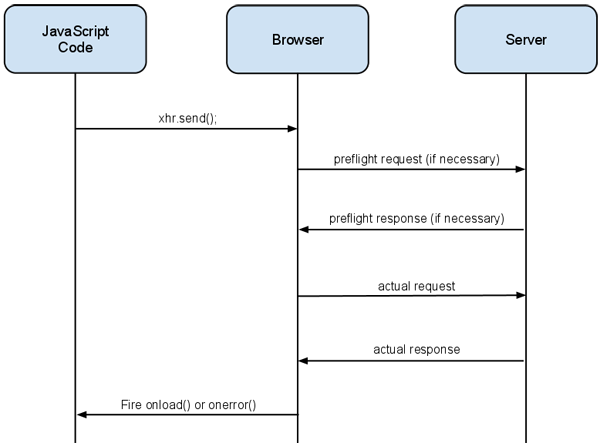
\includegraphics[scale=0.3]{img/CORS_FLOW.png}
	\end{center}
	\subsubsection{Web Messaging}
	\begin{itemize}
		\item Ermöglicht den Datenaustausch zwischen Dokumenten in anderen Tabs/Fenstern
		\item Senden: targetWindow.postMessage(message,targetURL)
		\item targetWindow = Referenz auf Zielfenster (Erhalt durch Öffnen des Fenster $\rightarrow$ return-Wert von window.open(); enthalten als contentWindow Property eines iframes)
		\item message = String oder Object das gesendet wird
		\item targetURL = URL des Zielfensters
		\item Empfänger implementiert onmessage-Handler $\rightarrow$ erhält ein Event mit den Attributen \textbf{data} (Inhalt der Nachricht), \textbf{origin} (URL des Senders) und \textbf{source} (Referenz auf das Sender-Fenster)
		\item Sicherheit
		\begin{itemize}
			\item Sender: Kann vertrauliche Daten an böses Ziel senden 
			\item Empfänger: Erhalte nicht vertrauenswürdige Daten aus böser Quelle
		\end{itemize}
	\end{itemize}
	\subsubsection{iframe Security}
	\begin{itemize}
		\item Inhalte können von Cross-Site über iframes eingebunden werden
		\item Problem: Fremde Site verändert eigene Site, Nutzer sieht nicht wer für den Inhalt verantwortlich, Site macht sich fremde Inhalte zu Nutze
		\item Lösung:
		\begin{itemize}
			\item sichtbar einbetten
			\item iframe busting (JavaScript der eingebetten Seite greift auf parent zu und schreibt sich auf höchster Ebene)
			\item Server setzt X-Frame-Options Header: \textbf{Deny }(komplettes Verbot), \textbf{Allow-From url} (Einbinden wenn Basisseite bestimmte URL) oder \textbf{Sameorigin} (Einbinden nur wenn Basisseite same origin ist)
		\end{itemize}
	\end{itemize}
	\subsubsection{Cross Site CSS}
	\begin{itemize}
		\item Einbinden von CSS von andere Seite
		\item Problem: Verdecken von Elementen, Unsichtbarkeit von Elementen, GUI redressing Attacken
	\end{itemize}
	\subsubsection{Cross Site Scripting}
	\begin{itemize}
		\item Definition: Webseite stammt aus einer Domain und lädt Skripte von einer anderen Domain
		\item WICHTIG: Cross Domain XHR verhindert durch Sandbox, Cross Domain Scripting wird nicht verhindert durch Sandbox
		\item Warum? Eigentlich wenig Sinn ausser bei Zugriff auf Mashup (Google Maps, Flickr Gallerie)
		\item Probleme: Fremdes Script zerstört Aussehen meiner Web Site völlig, Fremdes Script liest Werte aus Formularen aus, füllt Werte in Formulare ein oder modifiziert sie

		\item Bookmarklet = ist ein kleines in JavaScript geschriebenes Makro, das als Bookmark abgespeichert wird und dadurch die Funktionen eines Webbrowsers erweitert; Problem: laufen mit den Rechten der aktuell angezeigten Seite und können so Cookies-Stehlen und remote-Code hinzufügen
	\end{itemize}
	\subsubsection{Cross Site Request Forgery}
	\begin{itemize}
		\item Angreifer plaziert IMG-Link auf einer Seite mit Link welcher aufgerufen wird wenn Seite geladen wird
		\item Bsp: $\le$img src=\glqq http://bank.example/withdraw?account=bob\&amount=1000000\&for=mallory\grqq$\ge$
		\item Verteidigung: 
		\begin{itemize}
			\item nutzen von Logoff (Anfragen werden verworfen da Benutzer nicht angemeldet)
			\item Service nur als POST anbieten
			\item Zur Autorisierung auch ein Hidden Field nutzen
			\item Cookie double submission: Cookie und dazupassenden Teil in einem hidden field erwarten
		\end{itemize}
		\item Probleme:
		\begin{itemize}
			\item Cookies zur Vermittelung von Rechten (bei Aufruf wird Cookie verstandt); Erwünscht: Cross Domain User Tracking (Marketing), Unerwünscht: weil Cookies auch zum Speichern von User Credentials benutzt werden
			\item 2 implizite Annahmen im Link-Konzept: User sieht den Link, auf den er klickt aber er sieht nur Inhalt des Link-Tags nicht die URL $\rightarrow$ Betrug durch falsche GUI Konstruktion; User kennt den Effekt des Links, auf den er klickt aber URL namens abbuchen.php muss nicht abbuchen $\rightarrow$ Betrug durch vorgespiegelte URL Semantik
		\end{itemize}
	\end{itemize}
	\subsection{Konzeptuelle Probleme bei Berechtigungen}
	\subsubsection{Confused Deputy - Problem}
	\begin{itemize}
		\item Eine Komponente hat ein Recht aber das Recht wird genutzt, aber ausserhalb der erwarteten Verarbeitungssequenz oder ausserhalb des erwarteten Verarbeitungskontexts
		\item Eine Komponente referenziert eine andere Komponentee welche genutzt wird aber anders als mit der intendierten Semantik der Komponente
	\end{itemize}
	\subsubsection{Wie funktionieren Berechtigungen?}
	\begin{itemize}
		\item Owner Based Rights
		\begin{itemize}
			\item Objekte gehören einem User
			\item UserId hat bestimmte Rechte auf dem Objekt
			\item Programm hat unter einee UserId bestimmte Zugriffsrechte
			\item \textbf{Problem}: Kann Zugriffsrechte nicht mit anderen User teilen
			\item \textbf{Lösung}: Gruppenkonzept
		\end{itemize}
		\item Group Based Rights
		\begin{itemize}
			\item Objekte haben auch eine Gruppe
			\item User gehören in eine Gruppe
			\item User in einer Gruppe haben bestimmte Rechte
			\item \textbf{Problem}: Gruppenstruktur kann sehr komplex werden
			\item \textbf{Lösung}: Access Control Lists
		\end{itemize}
		\item Access Control Lists (ACL)
		\begin{itemize}
			\item Objekte haben eine ACL
			\item ACL weiss was welcher User darf
			\item \textbf{Problem}: Recht hängt nur vom User ab, nicht vom Programm oder Kontext des Programmes	
		\end{itemize}
		\item Capabilities
		\begin{itemize}
			\item Zugreifende Entitäten haben spezifische Fähigkeiten, auf Objekte zuzugreifen
			\item ???
		\end{itemize}
		\item Kontextuelle Restriktionen
		\begin{itemize}
			\item Bindung an den Kontext / die Seite / den Referer
			\item ???
		\end{itemize}
	\end{itemize}
	\subsubsection{Social Engineering}
	Social Engineering bedeutet den Missbrauch von gruppenspezifischen Verhaltensweisen um den Benutzer zu einer Handlung zu bewegen die er unter Kenntnis der damit verbundenen Folgen so nicht setzen würde
	\subsection{Fehlen von Trusted IO}
	\subsubsection{GUI Redressing Attacke}
	\begin{itemize}
		\item Attacke, welche durch eine versteckte Veränderung der Oberfläche erfolgt 
		\item Möglichkeiten: Cursordatei manipuliert
		\item Clickjacking: Stiehl Mausklick des Users (Angreifer spielt ihm vor, dass er auf eine andere Stelle klickt)
		\item Strokejacking: Stiehl den Tastendruck des Users (Browser sieht andere Taste als jene die der User gedrückt hat)
	\end{itemize}
	\subsubsection{Web Spoofing Attacke}
	\begin{itemize}
		\item Ziel: User vorzutäuschen auf einer anderen Seite zu sein als er tatsächlich ist (User denkt er ist auf bank.de, hat aber mafia.de aufgerufen)
	\end{itemize}
	\subsubsection{Injection Attacken}
	\begin{itemize}
		\item Techniken zur Generierung dynamischer Seiten erhalten Daten vom Client
		\item Techniken werden eingesetzt bei: SQL Queries, HTML Seiten, PHP Seiten, JavaScript Programme
		\item Beispiel: Einschleusen von HTML Code auf Webseite durch Formulardaten
		\item Beispiel: Manipulation des SQL-Query durch Manipulation im HTTP-Request
		\item Lösung: Validierung der Eingabe, Escapen von Quotes
	\end{itemize}
	\subsubsection{Covert Channel}
	\begin{itemize}
		\item ein parasitärer Kommunikationskanal, welcher Bandbreite (Informationskapazität) eines legitimierten Kommunikationskanals benutzt, um Informationen zu übermitteln.
		\item Stichwort: Steganographie
		\item Alle verdeckten Kanäle benötigen Bandbreite eines legitimierten Kommunikationskanals. Dadurch verringern sie entweder die Bandbreite des legitimierten Kanals oder laden ihm ohne Verringerung der Bandbreite weitere Informationen auf. Der verdeckte Kanal versteckt sich geschickt im legitimierten Kanal und ist somit schwer bis gar nicht zu entdecken.
		\item Speicherkanal (Storage channel) – Kommunikation über gespeicherte Daten.
		\item Zeitkanal (Timing channel) – Informationen werden über zeitliche Abfolgen informationstechnischer Verarbeitungen übertragen.
	\end{itemize}
	\section{Einführung in JavaScript}
	\subsection{Allgemein}
	\begin{itemize}
		\item Ziel: Dynamische Seiten ohne Server-Interaktion, Adaptive Webseiten mit rascher Reaktion auf Client-Interaktion, Rechenaufwand auf Client verteilen
		\item Lösungen: 
		\begin{itemize}
			\item JavaScript (Interpretierte Sprache)
			\item VB Script (MS Alternative zu JavaScript)
			\item Java Applets (Bytecode VM, eingebettet oder PlugIn)
			\item Active X (Kompilierte Programme auf Intel Architektur)
		\end{itemize}
		
		\item Später neue Anforderungen: Zugriff auf Hardware \& Sensoren (GPS, Webcam, Mic), Performane Boost durch clientseitige Parallelität und stärkere Kontrolle der User (App Stores, Binary Only Module)
		\item JavaScript kann: Zugriff auf Webseite+Header, Event Handler, Schnittstelle Java - JavaScript
		\item Vorteile von JavaScript:
		\begin{itemize}
			\item Extrem weites deployment
			\item Halbwegs uniform 
			\item Viele Client-seitige Libraries
			\item Beginnender Server-seitiger Einsatz (node.js)
			\item Homogenes Werkzeug auf Client \& Server
			\item Langsam etwas effizienter (Hotspot, V8, asm.js)
			\item Am Browser: Sicherer als Java \& ActiveX 
		\end{itemize}
		\item JavaScript ist: imperativ, objekt-orientiert, funktional, scripting Sprache (nicht funktional im Sinne von Haskell und Co, nicht oo wie C++ oder Java)
		\item Programmierer kann eigenen Programmierstil wählen d.h. wenig Zwang der Sprache 
		\item Nutzung als universelles Target, da sehr weit verbreitet (Jeder Browser kann JavaScript)
		\item Problem: JavaScript bietet wenig Garantien (keine Typsicherheit, wenig Abgrenzung der Module, Wenig Debug-Unterstützung, Wenig Optimierung)
		\item Lösung: Nachrüsten möglich 
		\begin{itemize}
			\item Typsystem: Typ-Annotation in Kommentaren dadurch bessere Analyse von Typsicherheit
			\item Optimierung: \\
			Sprachoptimierung nach der Analyse (Compiler von JavaScript nach JavaScript)\\
			Compilation auf eine VM
			\item Debugging: Firebug, Browser Konsolen (runtime) oder Closure Compiler (Compiletime)
		\end{itemize}

		\item JavaScript als:
		\begin{itemize}
			\item Imperative Sprache: Variablen, einfaches Typsystem, Ablaufsemantik usw... aber keine sinnvolle Abgrenzung von imperativen Sprachen möglich, da Variablen dynamisch getypt und anfänglich nicht kompiliert sind
			\item Funktionale Sprache: Funktionen, Rekursion, Funktionen als first-class-objects, anonyme Funktionen aber keine Seiteneffekt-Freiheit, kein komplexes Typsystem und keine referentielle Transparenz
			\item Objekt-orientierte Sprache: Klassen, Vererbung und Polymorphismus aber keine Namensräume, keine Zugriffsmodifikatioren, kein Typecasting und keine Templates
		\end{itemize}
	\end{itemize}
	\subsection{Funktionale Aspekte}
	\begin{itemize}
		\item Zugriff auf Parameter über Namen oder Array-Arguments (variadische Funktionen)
		\item Variadische Funktionen: Funktionen mit unbestimmter Arität (Zugriff oder Arraystruktur)
		\item Funktionsdeklaration und Rekursion wie üblich möglich
		\item Funktionen sind Werte (first-class-objects) d.h. können als Variablen gespeichert bzw. als Paramter übergeben werden
		\item Anonyme Funktionen Bsp: var quad = function (x) \{return x*x;\} (Funktion ist in quad-Variable gespeichert aber hat keinen Funktionsnamen)
		\item Closures: Anonyme Lambda-Definition mit freien Variablen (d.h. in der Funktion können Variablen genutzt werden, welche im inneren Kontext nicht bekannt sind)
		\item Eingebauter Compiler: Funktions-Körper oder beliebige Evaluation durch eval-Funktion
		\item Problem des Compilers: Langsam (da dynamisch) und gefährlich (geringe Kontrolle über Seitenveränderung)
	\end{itemize}
	\subsection{Objekt-orientierte Aspekte}
	\begin{itemize}
		\item Klassisch: Klassenbasierte Vererbung (Java,C++)
		\item In JS: Prototypenbasierte Vererbung
		\begin{itemize}
			\item Objekt besitzt Methode selber oder delegiert Suche an Prototyp
			\item Prototyp ist Eigenschaft der Klasse
			\item Methodensuche ist dynamisch und passiert zur Laufzeit
			\item Methoden können zur Laufzeit hinzugefügt werden
			\item Vererbungshierarchie entsteht zur Laufzeit
			\item Vererbungshierarchie kann zur Laufzeit dynamisch und mehrfach verändert werden
		\end{itemize}
		\item Jede Funktionsauswertung läuft in einem Kontext (this)
		\item Globales Objekt = Window 
		\item Erzeugtes Objekt = Konstruktor\\
		\textit{var dozent = new person (\glqq Gero\grqq);}
		\item Gebundenes Objekt mit call und apply
		\item In JavaScript gibt es keine Klassen. Es gibt jedoch Konstruktor-Funktionen (Konstruktoren) und prototypische Objekte.\\
		\url{http://molily.de/js/organisation-instanzen.html}
	\end{itemize}
	\subsection{Scripting-Aspekte}
	\begin{itemize}
		\item Dynamische Erweiterung: Attribute werden dynamisch generiert
		\item Es ist zulässig Variablen umzutypen
		\item Bietet Möglichkeit, alle Instanzvariablen zu iterieren (for (fieldnName in object) \dots)
	\end{itemize}
	\subsection{Weitere Aspekte}
	\begin{itemize}
		\item JavaScript Typen: schwach getypte Sprache (\textbf{typeof} prüft grundlegende Typen |primitiv oder Objekt| \textbf{instanceof} prüft auf Klasse eines Objektes) d.h. Variablen nicht getypt
		\item 3 Bestandteile von JavaScript
		\begin{enumerate}
			\item ECMAScript = standarditisierte Sprachkern von JavaScript (wesentliche Eigenschaften werden dort implementiert)
			\item Document Object Model = Sprachunabhängige API für HTML (\& XML, CSS) Dokumente und Baumstrukturen, kompletter Zugriff auf alle HTML Tags (innerHTML), den Stil (style und classname), Events via Event-Handler
			\item Browser Object Model = Stark Plattform-spezifische API für den Browser (window, document)
		\end{enumerate}
		\item Server-Side JavaScript: Interpretation und Verarbeitung von JavaScript auf Seiten am Server
		\item \textbf{V8} ist eine freie Implementierung der Scriptsprache ECMAScript (JavaScript) und soll die Ausführung von JavaScript-Code beschleunigen. Wird in C++ entwickelt und unterstützt Multicore.\\
		V8 steigert die Leistung zur Laufzeit, indem der JavaScript-Code bei der Ausführung durch so genannte Just-in-time-Kompilierung zunächst in nativen Maschinencode übersetzt wird. Weitere Leistungsvorteile ergeben sich aus Optimierungstechniken wie dem Einsatz von Inline Caching, das JavaScript-Objekte versteckt um geteilte Klassen erweitert, und einer so genannten „exakten automatischen Speicherbereinigung“, die Speicher schnell und in kleinen Portionen zuweist und wieder freigibt, was hierbei längere Wartezeiten vermeidet.
		
		\item Weiter Entwicklungen:
		\begin{itemize}
			\item CoffeeScript = knappes JavaScript, Postfix if Notation, Einrückungen (Python), Pattern Matching (Hasekll) $\rightarrow$ Compilation nach JavaScript (Problem: erzeugter JS Code schwer lesbar und debugging aufwendig)
			\item TypeScript = JavaScript für die große Systementwicklung, statisch getypte Variablen, Typ-Prüfung zur Compilezeit, echte Klassen usw
			\item Dart = JavaScript in C und Java erweitert (bisschen wie TypeScript)
		\end{itemize}
	\end{itemize}
	
	
	
	\section{JSON}
	\begin{itemize}
		\item JSON = JavaScript Object Notation
		\item Format für die Serialisierung von Objekten
		\item Unterstütze Datenstrukturen: Objekte, Arrays, Strings, Boolean, Integer, null
		\item Bewertung: kompakter als XML (weniger Overhead als XML, weniger aufwendiges Parsen), keine Attribute, keine DTD
		\item JSON Parse rund 10x schneller als XML Parse
		\item Einsatzbereiche: Server generiert JSON und Client generiert in JS aus JSON ein Objekt
		\item Risiko: Server sendet mehr als JSON Subset
		\item Erweiterung: JSONP (JSON + Padding)
		\item Padding (von englisch to pad ‚auffüllen‘) ist ein Fachbegriff der Informatik für Fülldaten, mit denen ein vorhandener Datenbestand vergrößert wird.
		\item Ermöglicht die Übertragung von (JSON-)Daten über Domaingrenzen
		\item Idee: 
		\begin{itemize}
			\item Client fordert ein bestimmtes Padding vom Server an
			\item Server führt Padding durch und liefert JSON + Padding aus
			\item Ergebnis wird als dynamisches Script Tag dem Dokument hinzugefügt
		\end{itemize}
		\item Ergebnis: Keine Restriktion hinsichtlich XHR same-origin, da Script Tag; JSON wird an richtiger Stelle in JavaScript eingebaut
		\item Erweiterung JSONRequest:
		\begin{itemize}
			\item Analog wie XMLHTTPRequest, aber kann aber nur JSON entgegennehmen
			\item keine same-origin Restriktion
			\item Effekt: Sicherer und flexibler; Kein Schaden, da nur Daten übertragen; Keine Restriktion
		\end{itemize}
	\end{itemize}
\section{JavaScript Pattern}
	\subsection{Scope Pattern}
		\textit{$\rightarrow$ äußerer Scope}\\
		function name() \{\\
		\textit{$\rightarrow$ innerer Scope}\\
		\};\\
		\textit{$\rightarrow$ äußerer Scope}\\
		\begin{itemize}
			\item innerer: 
			private instance \textit{var x = ...} oder 
			public instance \textit{this.y = ...}
			\item äußerer: 
			class property \textit{name.z = ...} oder
			generate inheritance \textit{name.prototyp = ...} oder
			modify inheritance \textit{name.prototype.u = ...}
			\item \textbf{Datenkapselung} bedeutet, dass das Erweitern des globalen Objekts sowie der DOM-Objekte auf ein Minimum reduziert wird. Ein Script sollte den globalen Scope nicht für seine Arbeitsdaten verwenden und globale Variablen möglichst vermeiden
		\end{itemize}
		\subsection{Module Pattern}
		\begin{itemize}
			\item We’ll simply create an anonymous function, and execute it immediately. All of the code that runs inside the function lives in a closure, which provides privacy and state throughout the lifetime of our application.\\
			(\url{http://www.adequatelygood.com/JavaScript-Module-Pattern-In-Depth.html})
			\item Mittels \textit{return} können Variablen/Methoden exportiert werden.
			\item Lexikalische Stabilität: 
			\begin{itemize}
				\item Optimierer (hier: Closure) können umbennen Bsp: \textit{numberOfStudents} in \textit{n}
				\item Wenn Optimierer den kompletten Code kennt unproblematisch, denn dann in allen Modulen konsistent umbenannt
				\item \textbf{1. Problem}: 2 separate Läufe des Optimierers auf Library und Nutzer der Library
				\item \textbf{2. Problem}: Optimierte Library und nicht-optimierter Code, der sie nutzt
				\item \textbf{Lösung} bei Closure: Quotes im JSON Rückgabe-Objekt verhindern Umbenennung durch Closure Compiler.
			\end{itemize}
		\end{itemize}
		\subsection{Revelation Pattern}
		\begin{itemize}
			\item Description: it is about having private methods, which you also expose as public methods
			\item Ähnlich wie das Exportieren im Module Pattern nur ohne return sondern durch Zuweisung im Körper (zu einer vorher definierten Variable im äußeren Scope)
		\end{itemize}
		\subsection{Anti-Pattern: Implizites Typecasting}
		\begin{itemize}
			\item Erscheint nicht im Quelltext
			\item potenzielle Fehlerquelle, wenn unabsichtlich verwendet 
			\item Bsp. binäre Operatoren
			 \begin{lstlisting}
(20 + 5) + "px"		// ist klar: "25px"
20 + (5 + "px") 	// ist klar: "205px"
20 + 5 + "px" 		// ist nicht so ganz klar !
			\end{lstlisting}
		\end{itemize}
		\subsection{Enforcing-New Pattern}
		\begin{itemize}
			\item Ohne das Erzwingen eines "new" bei der Objekterzeugung kann es zu Fehlverhalten kommen
			 \begin{lstlisting}
function Waffle() {this.tastes = "yummy";} // Konstruktor
// Problem: Vergessenes new:
var goodMorning = Waffle();
console.log(typeof goodMorning); 	// "undefined"
console.log(window.tastes); 		// "yummy"
			\end{lstlisting}
			\item Lösung
			\begin{lstlisting}
if (!(this instanceof Waffle)) {return new Waffle();}
			\end{lstlisting}	
		\end{itemize}
		\subsection{Nicht-Überschreibung}
		\begin{itemize}
			\item \textbf{Problem}: Kein Schutz des globalen Scopes vor Überschreiben
			\begin{lstlisting}
var MYAPP = {}; 		// unsicher, wenn MYAPP bereits existiert
if (typeof MYAPP === "undefined"){var MYAPP = {};} // besser aber aufwendig
var MYAPP = MYAPP || {}; 	// haeufig angetroffene Kurzform
			\end{lstlisting}	
		\end{itemize}
		\subsection{Chaining Pattern}
		\begin{itemize}
			\item \textit{obj.increment().add(3).shout();}
			\item Gestattet sehr kompakte, übersichtliche Programme und wird sehr oft in jQuery benutzt.
		\end{itemize}
		\subsection{Hinzufügen von Funktionalität}
		\begin{itemize}
			\item Anwendung des Chaining Pattern
			\item Erlaubt eine andere Weise Methoden für ein Objekt festzulegen 
			\begin{lstlisting}
if (typeof Function.prototype.method !== "function") {
	Function.prototype.method = function (name, implementation) {
	this.prototype[name] = implementation;
	return this;};
}
var Person = function (name) {this.name = name;}.
	method('getName', function () {return this.name;}).
	method('setName', function (name) {this.name = name;return this;
});
			\end{lstlisting}
		\end{itemize}
		\subsection{Browser-Weiche bei Initialisierung}
		\begin{itemize}
			\item Um eine Browser-Kompatibilität zu gewährleisten
			\item Bspw. kennt der IE \textit{window.addEventListener} nicht, sondern \textit{document.attachEvent} und ältere Browser verwenden \textit{utils.addListener}
		\end{itemize}
		\subsection{That}
		\begin{itemize}
			\item Because this frequently changes when you change the scope by calling a new function, you can't access the original value by using it. Aliasing it to that allows you still to access the original value of this. (\url{http://stackoverflow.com/a/4886696})
		\end{itemize}
	
	
	
	\section{Smallworld und Powerlaw Netzwerke}
	\begin{itemize}
		\item Ausgangsexperiment: Paket soll an eine Person geschickt werden, ausgehend von einer ausgewählten Person die nur den Name und der Region kannte des Empfängerns
		\item Vorgehen: Senden an eine Person von der man glaubt dass diese die Zielperson kennt
		\item Ergebnis: Manche Pakete erreichten ihr Ziel nicht aber wenn ein Paket sein Ziel erreichte,
		dann im Schnitt mit weniger als 6 Zwischenschritten
		\item Analogie: Routing im Internet\\
		(üblich: 20 und mehr Schritte Abstand)
		\item Ziel: Modellierung dieser Verhältnisse
	\end{itemize}
	\subsection{Erdös Netze}
	\begin{itemize}
		\item Erdös sehr aktiver Mathematik (und Graphentheoretiker)
		\item Erdöszahl:
		\begin{itemize}
			\item 0 = Erdös selber
			\item 1 = Koautor von Erdös (Person welche mit Erdös veröffentlicht hat)
			\item 2 = Koautor eines Koautor von Erdös 
			\item usw...
			\item Nicht jeder Mathematiker hat eine Erdös Zahl
		\end{itemize}
		\item Durchschnittliche Erdös-Zahl (über alle Mathematiker) ist kleiner als 5
		\item Persone-Netze
		\begin{itemize}
			\item Bsp: Xing, LinkedIn
			\item Es gibt viele Leute, welche noch keine Kontakte eingetragen haben
			\item Sobald es einen bestätigten Kontakt gibt, existiert mit großer Wahrscheinlichkeit ein Pfad zu dieser Person über andere Personen
			\item Bezeichung: Small World Phänomen
		\end{itemize}
	\end{itemize}
	\subsection{Systematische Charakterisierung von Small World}
	\begin{itemize}
		\item Problem = Unscharfe Definition (Wo beginnt Small World denn genau?)
		\item Grundidee: Die Welt sieht \glqq klein\grqq aus
		\item ungünstige Graphen haben zu viele/wenige Kanten
		\item Idee:
		\begin{itemize}
			\item Welt soll potentiell groß sein 
			\item Sie ist aber zu meiner Überraschung doch recht klein weil ich bei der Bewegung immer mal wieder auf Bekannte von Bekannten stoße
		\end{itemize}
		\item \textbf{Erstes Kriterium}: Sinnvolle Gesamtsituation
		\begin{itemize}
			\item Knotenzahl viel größer als Kantenanzahl pro Knoten
			\item Kantenanzahl pro Knoten viel größer log(Knotenanzahl)
		\end{itemize}
		\item Clustering Koeffizient eines Knoten
		\begin{itemize}
			\item Frage: Welcher Anteil der möglichen Verbindungen der Nachbarn untereinander ist tatsächlch im Graphen realisiert?
			\item Nahe bei 1: Die Nachbarn eines kennen sich gut untereinander (B)
			\item Nahe bei 0: Die Nachbarn eines Knotens sind einander meist fremd (A)
			\item \textbf{Interpretation des hohen Clusterkoeffizienten}: \glqq Wenn A den B kennt und A den C kennt, dann ist die Wahrscheinlichkeit hoch dass auch B und C miteinander zu tun haben
			\begin{center}
				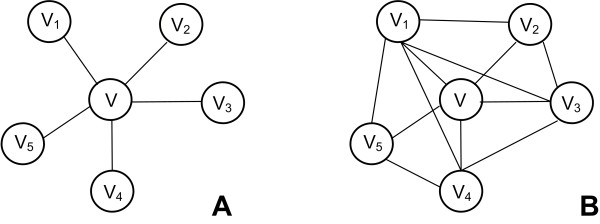
\includegraphics[scale=3]{img/cluster_koeffizient.jpg}
			\end{center}
		\end{itemize}
		\item Typische Entfernung (Mittlere minimale Pfadlänge)
		\begin{itemize}
			\item Beschreibt die minimale Länge eines Weges zwischen zwei Knoten, gemittelt über alle verbundenen Knotenpaaren
		\end{itemize}
		\item Randomisieren eines regulären k-Rings
		\begin{itemize}
			\item Regulärer k-Ring
			\begin{itemize}
				\item Nachbarn kennen sich untereinander sehr gut (regulär !)
				\item Mittlere Pfadlänge ist hoch (keine Fernverbindung)
			\end{itemize}
			\item Small World
			\begin{itemize}
				\item Nachbarn kennen sich untereinander sehr gut (noch gut lokal verankert)
				\item Mittlere Pfadlänge ist klein (da einige, aber wichtige Fernverbindungen)
			\end{itemize}
			\item Random 
			\begin{itemize}
				\item Nachbarn kennen sich untereinander sehr schlecht (Großstadtchaos)
				\item Mittlere Pfadlänge ist klein (da viele Fernverbindungen)
			\end{itemize}
		\end{itemize}
		\item \textbf{Zweites Kriterium}: Geringe Pfadlänge $\rightarrow$ Hinreichend viele globale Brücken
		\item \textbf{Small World Charakterisierung}
		\begin{itemize}
			\item Hoher Clusterkoeffizient: Gute, lokale Vernetzung
			\item geringe Pfadlänge: Hinreichend viele globale Brücken
			\item 6 degrees of separation-Eigenschaft: mit rein lokalem Wissen alleine eine gute, kurze Route finde
		\end{itemize}
		\item Ursachen für small world: Austauschstudenten, Gastprofessoren, Sommerurlaub\\
		$\rightarrow$ Randomisieren eines regulären k-Rings entspricht menschlicher Gesellschaft
	\end{itemize}
	\subsection{3 wichtige Netzklassen}
	\textbf{Hinweis:} Ein rudimentärer Generator der drei Netzklassen ist auf \url{https://github.com/Obererpel/network_classes} zu finden. 
	\begin{itemize}
		\item Idee zur Generierung: Initialer Graph durch Wachstumprozess werden neue Knoten und Kanten erzeugt, basierend auf einem Zufallsprozess
		\item 3 wichtige Graphklassen
		\begin{itemize}
			\item Erdös und Renyi (Gleichverteilung - Resultat: \glqq langweilig\grqq)
			\item Watts und Strogatz (Abnehmende Fernverbindungen - Resultat: Small World)
			\item Barabasi und Albert (Preferential Attachment - Resultat: Power Law)
		\end{itemize}
	\end{itemize}
	\subsubsection{Erdös und Renyi}
	\begin{itemize}
		\item Idee: Zufälliger Graph (Gleichverteilit)
		\item 2 Modelle:
		\begin{itemize}
			\item Zufälliger Graph: Unter allen möglichen Graphen mit n Knoten und e Kanten wähle einen zufällig auf Basis einer Gleichverteilung aus
			\item Zufällige Kante: Graph mit n Knoten, für jede Kante zwischen zwei Knoten wird mit der Wahrscheinlichkeit p realisiert
			\item Die zwei Konstruktions-Varianten unterscheiden sich \glqq nicht wesentlich\grqq
		\end{itemize}
		\item Verteilung der Knotengrade: Binomial-Verteilung
		\item Cluster Koeffizient: Recht klein
		\item Typische Entfernung: Abhängig von den Parametern
		\item Bewertung: unrealistisch, da nicht small world, zu kleiner Cluster Koeffizient für soziale Netze und keine Power Law Verteilung in Knotengraden
	\end{itemize}
	
	\subsubsection{Watts und Strogatz}
	\begin{itemize}
		\item Idee: Lokal regulärer Graph mit Fernverbindungen, Wahrscheinlichkeit der Fernverbindungen sinkt mit deren Länge 
		\item Lokale Konnektivität: jeder Knoten hat Kontakt zu allen Nachbarn der Schachbrettentfernung p
		\item Long Range Konnektivität: 
		\begin{itemize}
			\item Jeder Knoten hat zu weiteren q Knoten Kontakt
			\item Je weiter weg – umso unwahrscheinlicher
			\item Wahrscheinlichkeit ist dabei invers proportional zur Entfernug (Wahrscheinlichkeit = $\frac{1}{d^{r}}$)
			\item das Ziel ist es mit dem Parameter \textbf{r} die Größe des Clusters anzugeben
			\item Bei 2-dimensionalem Graph wäre r = 2 am besten, wobei r bestimmt die "Wanderaktivität" im Graphen
		\end{itemize}						 
	\end{itemize}
	
	\subsubsection{Albert und Barabasi}
	\begin{itemize}
		\item Idee: Preferential Attachment (Netz beginnt mit n Knoten, jeder neue Knoten verbindet sich zufällig mit alten Knoten, Wahrscheinlichkeit ist proportional zur Zahl der Kanten, die ein alter Knoten bereits hat)
		\item ALSO: Wer schon viele Verbindungen hat, kriegt noch besonders viele weitere (Monopole)
		\item \textbf{Konsequenz}: Knotengrad hat Powerlaw-Verteilung
	\end{itemize}
	
	
		\subsection{Das Power-Law}
	\begin{itemize}
		\item Die Potenzgesetze der Mathematik gehören zu den Skalengesetzen und beschreiben die Skaleninvarianz vieler natürlicher Phänomene.
		\item Ob eine gegebene Verteilung durch eine Potenzfunktion angenähert werden kann, zeigt sich bei einer doppelt-logarithmischen Auftragung. Ist der Graph der Funktion eine Gerade, so ist eine Näherung durch eine Potenzfunktion möglich. Die Steigung der Gerade ist dann ihr Exponent.
		\item Zipfsche Gesetz Verallgemeinert: Das \textbf{k}-häufigste Wort tritt $\frac{1}{k^{s}}$ so oft auf wie das häufigste
		\item Empirische Beobachtung: 80 – 20 Regel\\
		80\% der Einkommens in Italien werden von den 20\% Reichsten erzielt
		\item Scale Free Laws - Gesetzmäßigkeit: Verdoppelung der Filegröße reduziert Häufigkeit um Faktor vier 
		
	\end{itemize}
	\begin{center}
		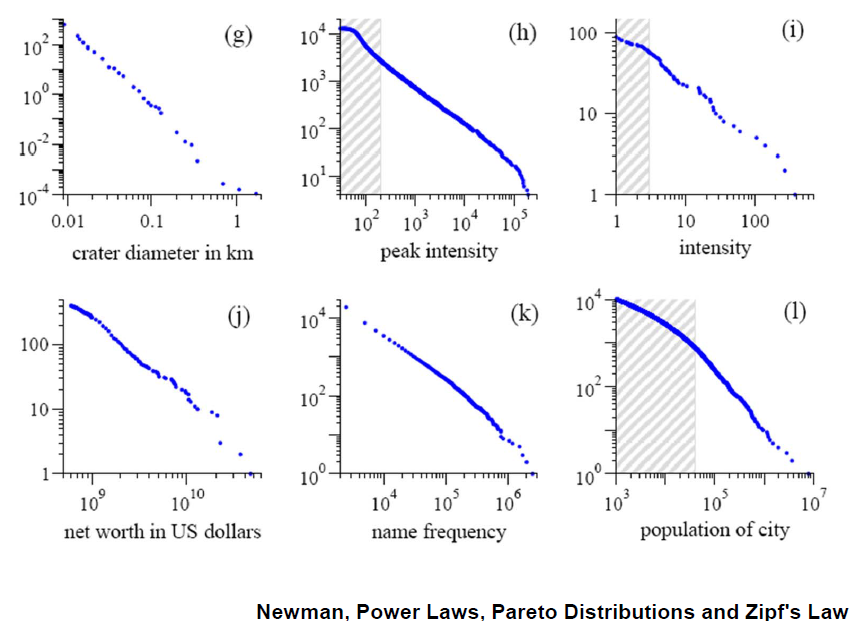
\includegraphics[scale=0.5]{img/power.png}
	\end{center}
	
	\subsection{Anwendungen im Web 2.0}
	\begin{itemize}
		\item Netzwerke mit Power Law Verhalten werden von 2 – 3 Big Players monopolisiert
		\item Folge: die Masse wird nicht gesehen und geht in der Bedeutungslosigkeit unter (Beispiel: Youtube)
		\item Modell des Long Tail
		\begin{itemize}
			\item Was ist besser? Sehr selten viel verdienen (forderer Teil der Kurve) oder sehr oft wenig zu verdienen (hinterer Teil der Kurve)
			\item These von Anderson: Sell more of less (Konzentriere Dich auf den Long Tail, da das Integral darüber sehr viele individuelle Nischen enthält)
			\item These von Pareto: 80\% des Effekts in 20\% der Produkte (Konzentriere Dich auf den Big Peak, nur da steckt die Masse drin) 
			\item Aktueller Stand: Pareto gilt (Emprisch belegt: Verkaufskurven steilen sich zunehmend noch auf
			Erziele 90\% des Verkauserfolgs mit 10\% der Produkte)\\		$\rightarrow$ Amazon(Alles!) vs. Thalia (Top 50 + Nachbestellen)
		\end{itemize}
		\item Annahme: Netzwerk besteht aus Knoten (Sites, Blogs, Artikel) und Kanten (Links); Netz wächst mit neuen Knoten und neuen Kanten; ein hoher Wert ergibt sich durch gute Verlinkung (Folge: hoher Google Page-Rank)
		\item Modell von \textbf{Erdös und Renyi} = Knoten werden zufällig ausgewählt – kann Power Law nicht erzeugen
		\item Modell von \textbf{Barabasi und Albert} = Preferential Attachment Modell (Wer hat dem wird gegeben d.h. neue Knoten verbinden sich zufällig mit ausgewähltem alten Knoten); Wahrscheinlichkeit fürs Verbindne steigt linear mit der Sichtbarkeit des alten Knotens $\rightarrow$ erzeugt Power Law Netzwerke
		\item Erhöhung der Sichtbarkeit:
		\begin{itemize}
			\item Technologie: Maximale automatische Verlinkung (Wikis, Blogs)
			\item Inhalt: Maximale aufreißerische Inhalte
			\item Prozeß: Maximale Interaktivität (Kommentare, Feedback)
		\end{itemize}
		\item es gilt also: \textbf{Zeichnet sich bereits ein Monopolist ab, so ist Konkurrenz zwecklos}
		\item Folgen und Probleme:
		\begin{itemize}
			\item Folge: Erzeugt hype-driven Content niederen Anspruchs im Boulevard-Stil für den Massenmarkt
			\item Folge der Folge: führt zu Monopolposition
			\item wer sich nicht an die Regeln hält bleibt unsichtbar, wer Regeln beachtet wird sichtbar (bzgl. hype-driven Content niederen Anspruchs im Boulevard-Stil)
			\item ABER: Statistische Modelle kennen keine Medienethik
		\end{itemize}
	\end{itemize}
	\section{DOM und DOM-API}
	\begin{itemize}
		\item Ziel: Veränderung des Dokumentes (Manipulation des Inhaltes oder Darstellung)
		\item Möglichkeiten:
		\begin{itemize}
			\item innerHTML-Eigenschaft: Inhalt eins Tags überschreiben
			\item Class und Style Modifikation: Attribute verändern wodurch Aussehen verändert wird oder neue Inhalte sichtbar
			\item JavaScript Dokumenten-Schnittstelle: document-Objekt in JavaScript ändern
			\item Multipart Mime Type: Mehrteilige Dokumente versenden und damit Inhalte updaten
			\item DOM-API: Direkte Manipulation der (semi)standardisierten OO-Darstellung des Dokuments
		\end{itemize}
		\item Initiatoren (Push/Pull):
		\begin{itemize}
			\item Server Side: Server will das sich der Inhalt ändert (Multipart Mime Type, Slow Load, Polling)
			\item Client Side: Durch Interaktion mit der Oberfläche wird Inhalt geändert (Meta Tag Refresh, XHR Request, JavaScript URL Wechsel (onload Handler))
		\end{itemize}
	\end{itemize}
	\subsection{innerHTML}
	\begin{itemize}
		\item HTMLElemente besitzen das Attribut innerHTML
		\item Lesen: Zeigt im Attribut enthaltenen HTML Text an
		\item Schreiben: Ins Attribut geschriebener Text wird als HTML geparst
		\item Beispiel: $<$div id=\grqq bsp\grqq$>$Etwas Text$<$/div$>$ (lesen)$\rightarrow$document.getElementById(\glqq bsp\glqq ).innerHTML = \glqq Nun $<$b$>$fetter$<$/b$>$
		Text\glqq 
		\item outerHTML: Enthält noch den Text des umschließenden Tags
		\item innerText: Text ohne Tags
		\item outerTags: wie innerTags aber ersetzt das komplette Element beim Überschreiben
	\end{itemize}
	\subsection{Class und Style Modifikationen}
	\begin{itemize}
		\item Class Modifikation:
		\begin{itemize}
			\item erlaubt Definition von Skins
			\item Dokument nutzt vordefinierte Class-Namen
		\end{itemize}
		\item Style Modifikation:
		\begin{itemize}
			\item erlaubt berechneten Style
			\item so Abhängigkeit von client-side Kontext möglich (Resize, Fenstergröße)
		\end{itemize}
		\item visibility und display Attribute:
		\begin{itemize}
			\item visibility: Element unsichtbar machen ABER Element bleibt an seinem Platz im Layout
			\item display: Element unsichtbar machen ABER Element wird aus dem Platz im Layout entfernt
			\item position: Absolute Positionierung oder relative Positionierung (bezgl. vorangehendem Element)
		\end{itemize}
		\item Problem: AJAX GUI ist oft dynamisch (Problem: Latenzzeit) $\rightarrow$ Lösung: Schaltbare GUI
		\item Schaltbare GUI: Alle Elemente einer GUI mit der HTML-Seite übertragen und bei User-Interaktion einfach zwischen den einzelnen Sichten umschalten $\rightarrow$ Realisierung durch visibility/display Attribute, z-Order Techniken oder Frame-Techniken
		\item n-stabiles Widget: hat n-stabile Zustände (Schalter mit 2 Positionen) $\rightarrow$ Implementierung durch Umsetzen von class-Werten
	\end{itemize}
	\subsection{JavaScript Dokumenten Schnittstelle}
	\begin{itemize}
		\item Ziel: Zugriff von JavaScript auf das Dokument in textueller Darstellung
		\item open(): öffnet Dokument zum Neubeschreiben
		\item close(): schließt Dokument
		\item write(): schreibt Text in das Dokument
		\item writeln(): schreibt Zeile in das Dokument
		\item Anwendung:
		\begin{itemize}
			\item Reines write: Ergänzt das Dokument (aber nur innerhalb des Dokuments, das gerade geparsed wird dh. innerhalb vn eingebetteten script-Tags)
			\item open-write-close Zyklus: schreibt in ein anderes Fenster aus einem fremden Dokument heraus (close nötig da sonst Browser das Dokument nicht lädt)
		\end{itemize}
		\item starke Einschränkung da nur Erweiterung des Dokument
		\item Einsatz bei: Live Query Responses, Webchat, Multi-Frame/Multi-Window Anwendungen
	\end{itemize}
	\subsection{Multipart Mime Type}
	\begin{itemize}
		\item MIME Type: Angabe des Dateityps in verschiedenen Internet Protokollen
		\item Syntax: \textit{Content-Type: multipart/mixed; boundary=separatorstring}\\
		(separatorstring taucht außer zur Trennung der Teile nicht auf)
		\item Beispiel:
		\begin{lstlisting}
MIME-Version: 1.0
Content-type: multipart/mixed; boundary=23xx1211
CRLF
--23xx1211
Content-type: text/html
CRLF
Erster Teil (HTML Daten)
--23xx1211
Content-type: audio/aiff
CRLF
Zweiter Teil (Audio Daten)
--23xx1211--
		\end{lstlisting}
		\item Arten:
		\begin{itemize}
			\item Multipart/x-mixed-replace (ankommende Teil ersetzt den angezeigten Inhalt)
			\item Multipart/form-data (Für komplexes Upload bei POST bei Forms; Jedes Element des Forms wird als separater Teil einer Multipart Nachricht codiert; Server erhält aber nur eine einzige Nachricht)
			\item Multipart/related (Bspw. Mail mit Inline-Bildern)
		\end{itemize}
	\end{itemize}
	\subsection{DOM Api}
	\begin{itemize}
		\item DOM enthält Dokumententteile in OO Baumstruktur (einsehbar: Firebug, Chrome, Dom Inspector)
		\item DOM-Api erlaubt diese OO Sicht zu modifizieren (Finden,Löschen,Erzeugen,Append,Preprend,Inhalt modizizieren, Attribute modifizieren)
		\item Zugriff aus JavaScript
		\item Wichtige Funktionen:
		\begin{itemize}
			\item createElement: erzeugt einen Knoten
			\item setAttribute: setzt einen Attributwert (Zugriff meistens auch über JavaScript Property möglich)
			\item setNodeValue: setzt den Textwert eines Knoten
			\item appendChild: fügt einen Knoten an eine Liste von Kindern
			\item removeChild: entfernt ein Kind
			\item replaceChild: ersetzt ein Kind
		\end{itemize}
		\item Vorteil: robuste API, flexibel, Standardisiert
		\item Nachteil: hoher Funktionsaufwand für kleine Änderung, relativ langsam 
		\item Probleme:
		\begin{itemize}
			\item Browser-Abhängigkeiten: Unterschiedliche Implementierung $\rightarrow$ Verschiedenen Code ausliefern nach User Agent Header; Dynamisch erkennen und Code ansteuern
			\item Flackern beim Neuaufbau $\rightarrow$ Unsichtbar schalten+Aufbauen+Sichtbar schalten
		\end{itemize}
	\end{itemize}
	\subsection{Slow Load}
	\begin{itemize}
		\item alias: Reverse Ajax, Comet
		\item Idee: Offenhalten einer Verbindung durch sehr langsame Server
		Server-Response
		\item Ziel: Server will den Client informieren das was passiert ist
		\item Umsetzung: 
		\begin{itemize}
			\item Slow load aus einem Hidden Frame/IFrame angefordertn – bleibt damit unsichtbar
			\item Slow load liefert keine Daten oder Daten mit "NOP"-Semantik, bis der Server dann wirklich etwas vom Client will
		\end{itemize}
		\item Realisierungen:
		\begin{itemize}
			\item Script-Tag Slow Load: Will der Server etwas vom Client, sendet script-Tag die bei Ankunft am Client verarbeitet wird
			\item XHR Slow Load: Server zögert die Antwort auf einen XHR lange hinaus
		\end{itemize}
		\item Nachteil: Server muss Kommunikationskanal offen halten, skaliert schlecht
	\end{itemize}
	\subsection{Polling}
	\begin{itemize}
		\item Idee: Client fragt Server regelmäßig ob was passiert ist
		\item Ziel: Cliet will wissen ob was passiert ist
		\item Nachteil: unnötige Belastung, skaliert schlecht, erhöht Latenzzeit durch dauerhafte Anfragebehandlung
	\end{itemize}
	\subsection{Metatag Refresh}
	\begin{itemize}
		\item Idee: Das Refresh Meta-Tag kann ein reload derselben URL auslösen
		\item Sollte serverseitig durch Status-Tracking (Bsp: Cookie) unterstützt sein.
		\item Angabe im HTML-Dokument dass das Dokument regelmäßig neu geladen wird
		\item Erweiterung um redirect
	\end{itemize}
	
	
\section{Serverseitige Performance}
	\begin{itemize}
		\item Probleme:
		\begin{itemize}
			\item Webserver mit 10k und mehr Connections pro Sekunde
			\item Problem wird schwerer durch W2.0 stärker fragmentiertes Web (Mehr Ressourcen (Bilder, CSS, JS), mehr Kanäle (Websockets), häufigere Interaktion (Responsive Web))
		\end{itemize}
		\item Lösungen: Effizientere Nutzung der Protokolle
		\begin{itemize}
			\item Persistente Verbindugen: mehere http-Requests pro tcp-Verbindung (Sockets)
			\item Request Pipelining: Mehere Requests statt stop-and-wait (mehere Anfragen senden anstatt auf Antwort auf einzelne Requests zu warten)
			\item Parallele Verbindungen: Mehere parallele tcp-Verbindungen
			\item Preloading: früh laden und damit Ressourcen schon vorhanden wenn benötigt
			\item Caching: nur einmal laden und wieder verwenden
			\item Chunked Transfer: Übertragung von kleinen Teilen sobald bereit
			\item Rohe Komprimierung: zip auf den Inhalten
			\item Smarte Komprimierung: BSON (Effizienten Encoding von JSON), ProtoBuf (BSON von Google)
			\item Websockets: Socket für http-Requests (weniger header overhead)
			\item SPDY und HTTP 2.0: neue Header für Steuerung\\
			(Weiterentwicklung und Verbesserung des http Protokolls durch Google)
		\end{itemize}
	\end{itemize}
	\subsection{SPDY und HTTP 2.0}
	\begin{itemize}
		\item Ziele:
		\begin{itemize}
			\item Reduktion der Latenz
			\item bessere Nutzung der Bandbreite
			\item neue Konzepte: Server Pushing und Hinting, Priorisierung, TCP Multiplexing
			\item Weitgehende Rückwärtskompatibilität
			\item Nahtloses, dynamisches Upgrading
		\end{itemize}
		\item Multiplexing: alle Requests über eine TCP Verbindung\\ (dadruch nur einmaliges 3way Handshaking Aufwand - Syn, SynAck, Ack)
		\item Server Pushing: Server sendet Ressource, ohne dass Client schon requestet hatte
		\item Server Hinting: Server informiert Client das best. Ressource nötig sein wird; Client überpüft ob im Cache wenn nicht dann Request
	\end{itemize}
	\subsection{Ressourcen Vergabe}
	\begin{itemize}
		\item ???
	\end{itemize}
	\subsection{Node.js}
	\begin{itemize}
	\item Grundsätzlich: Server-Side JavaScript ermöglicht Interpretation und Verarbeitung von Seiten am Server
		\item I/O Framework für Serverside JavaScript(V8-Basis, Nutzt event based programming und epoll)
		\item Vorteil: sehr kompakte Server, sehr leistungsfähig bei hohen Connection, Reduziert Anzahl Technologiebrüche in Web Anwendungen (nur eine Sprache für Client und Server)
	\end{itemize}
\section{Privatheit}
	\begin{itemize}
		\item \glqq \textbf{Privacy in Private}\grqq: Grundsätzliches Recht auf Privatheit
		\item \glqq \textbf{Privacy in Public}\grqq: Informationelle Selbstbestimmung (jeder hat das Recht selbst zu entscheiden welche Daten über sich von anderen gebraucht werden und welche Daten auf einen selbst einwirken dürfen)
		\item Paneopticum: rundes Gefängnis auf Cuba
		\item \glqq \textbf{Interpersonal Privacy} \grqq: Austausch von Informationen so, daß es maximal sozial nützlich
		erscheint (Facebook, Privatheit als ökonomisches Gut das getauscht werden kann)
		\item \glqq \textbf{Zero Privacy}\grqq: Privatheit als verloren gegangene Eigenschaft
		\item \textbf{digitales Panoopticon}: Datensammlungen führen allein durch ihr Bestehen bereits zu einer Verhaltensänderung\\
		(Beispiel Augen-Plakate
	\end{itemize}
	\subsection{Verlust der Privatheit}
	\begin{itemize}
			\item Im ökonomischen Raum durch Erstellung von Profilen (Amazon, Google)
			\item Im öffentlichen Raum durch Registrieren abweichenden Verhaltens (FBI, BND)
			\item Im sozialen Raum durch den Massenwahn der Selbstpreisgabe (Facebook,G+)
			\item Im digitalen Raum durch digitaler Angreifer
	\end{itemize}
		\subsection{Erstellung von Profilen}
	\begin{itemize}
		\item Wofür: Marketing, Cookie-Pricing, Reidentifikation des Browsers
		\item Wodurch: Cookies, Session
		\item Ziele:
		\begin{itemize}
			\item Antwort auf die Frage: \glqq Welche Zielgruppe reagiert auf welche Reize?\grqq (Neuromarketing)
			\item Möglichst hohe Einnahmen (bspw. buchen von Flügen/Autos)
		\end{itemize}
	\end{itemize}
		\subsection{Registration abweichenden Verhaltens}
	\begin{itemize}
		\item komplizierte Darstellung des Konflikts
		\item Wofür: Die Suche nach den Bösen
		\item Wodurch: Defekte \& Unerwünschte Software \& Der NSA ANT Catalogue\\
		(Stecker Manipulation, Packete öffnen und anpassen,
	\end{itemize} 
		\subsection{Selbstpreisgabe im (digitalen) sozialen Raum}	
	\begin{itemize}			\item \textbf{Bewusst}: In sozialen Netzen
		\item \textbf{Fahrlässig}: In weiteren digitalen Räumen
		\item \textbf{Heimtückisch}: Durch Instrumentierung
		\item \textbf{Beispiel}: Sexuelle Orientierung aus Freunde-Netz
		\item Facebook: \glqq If your're not paying for it, your're not the customer. You're the product being sold.\grqq
		\item RFID-Chips, Cloud, Geräte-Finder, iPhone als Ortungswanze, Webcam,...
			
	\end{itemize}
		\subsection{Digitale Angreifer}
	\begin{itemize}
			\item Bsp. Dropbox Passwörter (Software Komplexität); Zertifikate (Schlamperei bis Kooperation)
			\item Zerodays: Der Markt unentdeckter Fehler
			\item Software Qualität: Fehler pro Tausend Programmzeilen
			\begin{itemize}
				\item Gut: 1 – 10 Fehler (20 – 100 USD / Programmzeile) Bsp: Betriebssystem
				\item Sehr gut: Weniger als 0.5 Fehler (Rund 1.000 USD / Programmzeile) Bsp: Space Shuttle				
			\end{itemize}
	\end{itemize}
		\subsection{Privacy International}
	\begin{itemize}
		\item Menschenrechtsorganisation mit Sitz in London beobachtet weltweite Entwicklung der Privatheit $\rightarrow$ Ausmaß von Privacy Verletzungen und Rückgang von privacy ist erschreckend
	\end{itemize}
		
		\subsection{Privacy enhancing Technology}
		(Technologie, welche die Privatheit des Benutzers verbessert)
	\begin{itemize}
		\item Anonyme Kommunikation
		\item Zero Knowledge Protokolle\\
		(Beweisen, dass man etwas weiß – ohne das Wissen zu verraten)
		\item Verteilte Protokolle\\
		(Wenn man einem nicht vertraut – auf mehrere Schultern verteilen)
		\item Minimale Transaktionserfordernisse\\
		(System so designen, dass nur minimale Daten erforderlich sind)
	\end{itemize}
			\subsubsection{Anonyme Kommunikation}
			\begin{itemize} 
				\item Teilinformationen eines Kommunikations-Akts, die miteinander verbunden werden können
				\begin{itemize}
					\item Zeitpunkt des Sendens / Empfangens
					\item MAC Adresse / IP Adresse des Senders / Empfängers
					\item Bürgerliche Identität des Senders / Empfängers
					\item Inhalt der Kommunikation
					\item Bezug zu anderen Kommunikationsakten
					\item Profil: Kaufverhalten, politische Überzeugung, Muttersprache usw. von Beteiligten
					\item Co-Daten: Person zählt zur selben Gruppe wie eine andere Person
				\end{itemize}
				\item Begriffe: \textbf{klassisches Pseudonym} (Nick aber nicht die bürgerliche Identität bekannt) \& \textbf{Linkable Pseudonym} (Nick und bürg. Name sind unbekannt, es ist nur bekannt, dass die Person bspw. 2 Posts geschrieben hat) \& \textbf{Anonymität}
				\item Die \textbf{Anonymitätsmenge} ist die Menge der Personen, von denen die gesuchte Person aufgrund der vorliegenden Daten nicht getrennt werden kann.
				\item Tor
				\begin{itemize}
					\item Basiert auf Kaskaden
					\item Probleme: 
					\begin{itemize}
						\item Wie findet man zuverlässige Tor Relays?
						\item Information Leakage durch Browser
						\item Globale Traffic Analyse
					\end{itemize}
					\item \textbf{Timing Analyse} bei kleiner Anonymitäts-Menge und geringem Traffic führt bei geringer Latenz-Zeit zu rascher Enttarnung des Benutzers durch einen Angreifer mit Fähigkeit zur (globalen) Verkehrs-Analyse.
					\item Bequemlichkeit Problem:
					\begin{itemize}
						\item Anonymitäts-Software macht Aufwand
						\item Wird daher nur für "heikle" Inhalte genutzt
						\item Daher ist jeder verdächtig, der sie nutzt
						\item Nutzung von Anonymitäts-Software führt bereits zu weiterer Überwachung
						\item Die Anonymitätsmenge ist immer sehr klein
					\end{itemize}
					\item Bequemlichkeit Lösung: Wir nutzen alle jederzeit Anonymitäts-Software $\rightarrow$ Die Anonymitätsmenge wird sehr groß  $\rightarrow$  Die Wirksamkeit des Schutzes wird besser $\rightarrow$ Die Software wird immer besser
				\end{itemize}
			\end{itemize}
			\subsubsection{Zero Knowledge/ Secret Splitting/ Secret Sharing}
			\begin{itemize} 
				\item funktioniert bei NP-Vollständigen Problemen
				\item Bspw. Nutzen eines Polynoms 6. Grades: bei 0 wird der geheime Wert angezeigt $\rightarrow$ Es werden 7 von mglweise 9 Punkten benötigt $\rightarrow$ Deshalb an andere verteilen, da alleine keine Aussage getätigt werden kann.
			\end{itemize}
			\subsubsection{Minimale Transaktionserfordernisse}
			\begin{itemize} 
				\item ???
			\end{itemize}
\section{Attention Economy}
	\begin{itemize}
		\item Agrargesellschaft $\rightarrow$ Industriegesellschaft $\rightarrow$ Wissensgesellschaft (Wie komme ich möglichst schnell and möglichst viel Information?)
		\item Was ist jetzt der \textbf{limitierende Faktor}?\\
		(CPU Leistung?, Bandbreite?, Mobile Erreichbarkeit?, Speicherplatz?, Inhalte?, Stromverbrauch?, Preis?)
		\item Der wesentliche Engpass ist gegeben durch:
		\begin{itemize}
			\item Zeit
			\item Menschliche intellektuelle Verarbeitungsgeschwindigkeit
			\item Aufmerksamkeit
		\end{itemize}
		\item Aufmerksamkeit ist ein wertvolles Gut, folglich ist das Erregen von Aufmerksamkeit Diebstahl xD
		\item Problem: Aufmerksamkeit erregen und \textbf{halten} (Als Informatiker aus einer anderen Perspektive als sonst als \glqq Opfer\grqq
	\end{itemize}
	\subsection{Aufmerksamkeit als limitierender Faktor}		
	\begin{itemize}
		\item minimale Eintrittsbarieren mit asymptotisch Null Fertigungskosten
		\item Viele Probleme (zu) gut gelöst: Auswahl, Suche, Finden
		\item Wir ertrinken in Informationen (bzw. besser: Daten)
		\item Wir diskutieren Attention Deficit Syndrome als Krankheit
		\item Immer intensiverer Wettbewerb um Aufmerksamkeit\\
		(Bsp: Suchmaschinen Ranking, Web Einschaltquoten, TV Einschaltquoten, Gratis-Handy, gratis Suchmaschine, gratis Web-Portal)
		\item Aufmerksamkeits-Personen erhalten mehr Ressourcen als Fähigkeits-Personen
		\begin{itemize}
			\item Bsp: Früher: Generäle und Staatsmänner werden Politiker
			\item Bsp: Heute: Schauspieler und Medienjongleure werden Politiker
		\end{itemize}
		\item Davenport \& Beck verstehen das \glqq Attention Deficit Syndrome\grqq als Krankheitsbild einer Institution / der Gesellschaft - Merkmale:
		\begin{itemize}
			\item Kaum Zeit für längere Reflexion (bspw. Studienzeitverkürzung)
			\item Probleme, die Aufmerksamkeit des Gegenüber längere Zeit einzufangen (Aufmerksamkeit via animierter Multimediapräsentationen)
			\item etc.
		\end{itemize}
	\end{itemize}		
	\subsection{Psychologische Faktoren}
	\begin{itemize}
		\item Geteilte Aufmerksamkeit: Keine Gefahr übersehen \& Keine Chance verpassen
		\item Maslov Pyramide: Evolution zwingt uns viele Gefühle auf, deren Wahrnehmung lebenswichtig sein kann. Diese werden außerhalb der konkreten Wahrnehmung aber wieder schwer vorstellbar\\
		
		\url{http://www.topfox.ch/wp-content/uploads/maslow\_beduerfnispyramide\_gross-1024x721.png}
		
	\begin{center}
		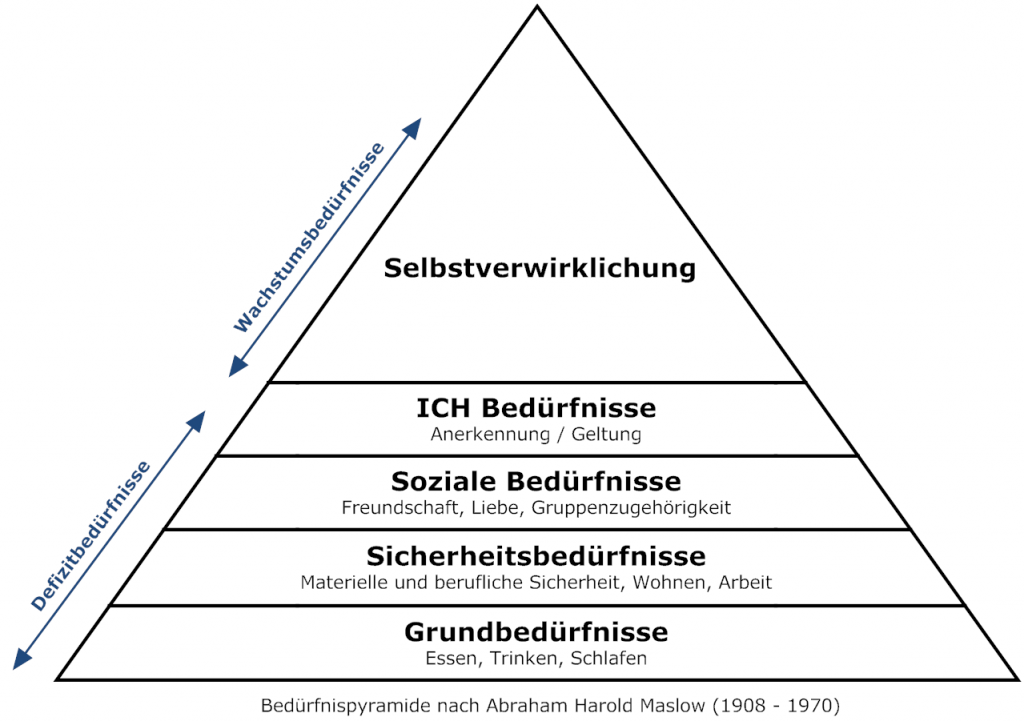
\includegraphics[scale=0.3]{img/maslow.png}
	\end{center}
		\item Ein Wechsel der Aufmerksamkeit ist prinzipiell extrem schnell möglich und kann durch äußere Faktoren erzwungen werden: Ist physiologisch \& psychologisch höchst belastend		
	\end{itemize}	
	\subsection{Dunbar Zahl}
	\begin{itemize}
		\item Viele Spezies bilden sozialen Netze und die Dunbar Zahl beschreibt die Größe der sozialen Netze einer Spezies
		\item Limitierende Faktoren sind:
		\begin{itemize}
			\item Neuronale Fähigkeit einen emotionalen Zustand mit einem Wesen zu assoziieren
			\item Zeit und materielle Ressourcen zur Pflege des Netzwerks
		\end{itemize}
		\item Idee: Dunbar Zahl skaliert mit Größe des Neurocortex $\rightarrow$ Menschliche Dunbar Zahl bei 150
	\end{itemize}
	\subsection{Arten der Aufmerksamkeit nach Davenport \& Beck}
	\begin{itemize}
		\item \textbf{Freiwilligkeit} der Aufmerksamkeit
		\begin{itemize}
			\item Captive Aufmerksamkeit (Flash, animated GIF, Popup Screen)
			\item Freiwillige Aufmerksamkeit (Hauptdokument, das ich gerade geöffnet habe)
		\end{itemize}
		\item \textbf{Motivationsart} der Aufmerksamkeit
		\begin{itemize}
			\item Attraktive Aufmerksamkeit (Dinge, die ich anstrebe)
			\item Aversive Aufmerksamkeit (Dinge, die ich vermeiden will)\\
	$\rightarrow$ Aversive Aufmerksamkeit ist stärker: Only bad news is good news		
		\end{itemize}
		\item \textbf{Bewusstheit} der Aufmerksamkeit
		\begin{itemize}
			\item Vordergründige Aufmerksamkeit ist explizit, fokussiert, bewusst (Steuererklärung,Masterarbeit, Telefongespräch beim Autofahren)
			\item Hintergründige Aufmerksamkeit ist implizit, unfokussiert, unbewußt (Autofahren obwohl dabei auf Telefonat achte)
		\end{itemize}
		\item Eigenschaften von Aufmerksamkeit
		\begin{itemize}
			\item Schwer objektiviert meßbar
			\item Stark volatil (Kann instantan verschwinden)
			\item Nicht virtualisierbar: Kein Ausborgen und Zurückgeben, kein Ansparen \& Zins
			\item Handelbar (Wird gegen Geld getauscht, aber meist nur mittelbar Bsp: Amerikanisches Gratis-TV mit Werbefinanzierung)
			\item Leicht manipulierbar (Unterliegt nur teilweise dem bewußten Wollen)
		\end{itemize}
	\end{itemize}
	\subsection{Wie hält man Aufmerksamkeit?}
	\begin{enumerate}
		\item Make a Change
		\begin{itemize}
			\item Dauernde kleine Änderungen halten die Aufmerksamkeit wach
			\item Bsp: Schnelle Schnitte in Filmen, neue Webseiten, rascher Themenfluss in Blogs,...
		\end{itemize}
		\item Ein- und Ausstiegspunkte sowie Wiedereinstiegspunkte vorsehen
		\begin{itemize}
			\item Bsp: Web erlaubt freien Wechsel der Aufmerksamkeit (besser als der 500 Seiten
Roman)
			\item Bsp: Bücher sind in Kapitel strukturiert
			\item Bsp: Filme sind in Serien aufgeteilt
		\end{itemize}
		\item Relevanz
		\begin{itemize}
			\item Inhalte betreffen mich und erfüllen ein Bedürfnis
			\item Inhalte wechseln oft, erfüllen aber immer wieder mein Bedürfnis
			\item Kontinuierlicher Strom von Neuigkeiten
		\end{itemize}
		\item Community
		\begin{itemize}
			\item Vermittelt ein Gefühl des "Ownership"
			\item Hat Mechanismen der Partizipation und Co-Creation
			\item Erlaubt Anpassung, Individualisierung
			\item Befriedigt Mechanismen persönlicher Eitelkeit
			\item Bsp: Blogs, Soziale Portale
		\end{itemize}
		\item Stakeholder-Prinzip = User Investment
		\begin{itemize}
			\item Wenn der Benutzer Energie (Zeit, Geld) investiert hat, bleibt er interessiert
			\item Bsp: Aufgebaute Reputation (Forengott), Gepflegtes Profil oder Datenbestand, Gespeicherte E-Mails
		\end{itemize}
		\item Convenient
		\begin{itemize}
			\item Schnell, Intuitiv, Bedienerfreundlich, Information in wohlproportionierten Häppchen, minimale Ablenkung
		\end{itemize}
	\end{enumerate}
	\subsection{Die 4 Muster der Aufmerksamkeit}
	\begin{enumerate}
		\item Adaptieren
		\begin{itemize}
			\item \textbf{Adaptieren}: Die Umgebung, der man begegnet, individueller auf sich abstimmen, und dadurch die Impedanz in der Begegnung mit der Umgebung reduzieren
			\item \textbf{Mechanismen:}
			\begin{itemize}
				\item Personalisieren (Ich selber)
				\item Recommender (Algorithmen berechnen Passung aus Clusterung von Verhaltensparametern)
				\item Peers (Meine Bezugsgruppe in Familie, Arbeitsplatz, Branche, Verein)
				\item Virtuelle Peers (Bezugsgruppe, in die ich zu einem bestimmten Thema statistisch am besten hineinpasse)
			\end{itemize}
		\end{itemize}
		\item Sozialisieren
		\begin{itemize}
			\item Mechanischer Türke (Komplexe Aufgaben an Maschine durch Mensch gelöst statt durch Maschine)\\
			Bspw. Amazon mechanical turk
			\item Hier: Automatisieren von Bewertung, Hilfestellung, Feedback, Kategorisierung, Verlagern von Feedback
		\end{itemize}
		\item Auswählen/Filtern
		\begin{itemize}
			\item Selektive Nutzung statt linearer oder extensiver Nutzung
			\item Trend: Erleichtere dem User selektive Nutzung durch Navigationsangebote
			\item Antitrend: Zwinge die Aufmerksamkeit des Nutzers
			\item \textbf{Filtern}: Verhindern, daß unerwünschte Inhalte meine Aufmerksamkeit beanspruchen - Bsp: Ad Blocker, Spam Filter
			\item \textbf{Kondensationsprozess} in der Entscheidungsbasis
			\begin{itemize}
				\item Viele Allokations-Entscheide, daher wenig Ressourcen für Einzelentscheid
				\item Bsp: Subject bewirkt eMail Lese-Entscheid (bei unbekanntem Sender)
				\item Bsp: Lead-Texte und Media-Previews bewirken Nutzungsentscheide
			\end{itemize}
		\end{itemize}
		\item Lenken
		\begin{itemize}
			\item Durch eine Maschine
			\begin{itemize}
				\item \textbf{Fremdbestimmt}, ich habe wenig Einfluß auf den Mechanismus (Google:Pagerank bestimmt)
				\item \textbf{Eigenbestimmt}, ich lege Kriterien für Maschine fest( Whitelist, Blacklist für Mailer)
			\end{itemize}
			\item Durch den Menschen\\
			(Medienproduzenten, Medienkonsumenten, Community)
			\item Kaptive versus freiwillige Aufmerksamkeit
			\begin{itemize}
				\item \textbf{Initiale Aufmerksamkeit}: Einstieg über Kondensatoren\\
				(Bsp: Brand Recognition - Initiale Geschäftspolitik von Amazon)	
				\item \textbf{Initiale Aufmerksamkeit}: Einstieg über Verkehrslenkungs-Seiten\\
				(Bsp: Suchmaschinen - Market Cap von Google)
				\item \textbf{Weiterleitung}: Prognose von Bedürfnissen\\
				(Bsp: Recommender - Cobuy, Cocitation)
			\end{itemize}
		\end{itemize}		
	\end{enumerate}
	\subsection{Folgen für Technologie und Anwendung}
	\begin{itemize}
		\item Aufmerksamkeit wird wesentliches Kriterium in SW-Akzeptanz
		\begin{itemize}
			\item Weg von \glqq SW soll wenig kosten\grqq hinzu \glqq soll wenig Aufmerksamkeits-Kosten verursachen\grqq
			\item Spam Blocker, Ad Blocker, Zero-installation, auto-update, zero-configuration, ASP, AJAX – Lösungen
		\end{itemize}
		\item Aufmerksamkeit wird zentrale Modalität in Anwendungen
		\item These: Für optimale Aufmerksamkeits-Allokation brauchen wir soziale Software
		\begin{itemize}
			\item Erlaubt dem Anwender direkte Interaktion mit seiner Peer Group
			\item Ermöglicht dem Benutzer, eigene Peer Groups zu bilden
		\end{itemize}
	\end{itemize}
	\subsection{Business Aspekte}
	\begin{itemize}
		\item Produkte und Dienstleistungen (Fokus umfasst nur das \glqq Ding an sich\grqq)
		\item Bedürfnisse
		\begin{itemize}
			\item Bsp: Mobilität
			\item Fokus umfasst komplexes Bedürfnis und damit auch Schnittstellen (Bsp: DB Bahnfahrt \& Car Pool)
			\item Anforderungsdefinition des Kunden (Bsp: Will von A nach B)
		\end{itemize}
		\item Kundenbindung
		\begin{itemize}
			\item Wird dem Kunden vorgegeben und dieser kann schwer wechseln – hohe Switching-Kosten
			\item Fehlentscheidung kommt Kunden teuer, kleine Adoption Rate
		\end{itemize}
		\item Kundenzufriedenheit
		\begin{itemize}
			\item Kann vom Kunden gewählt werden und dieser kann leicht wechseln\\
		$\rightarrow$ Kunde will nicht wechseln, wenn Struktur wählen			 kann, die er will\\
		$\rightarrow$ Geringere strukturelle Bindung, höhere faktischer Bindung
		\end{itemize}
		\item Mögliche Folgen
		\begin{itemize}
			\item Bekannt: Hochpreispolitik \& Diebstahl beim Kunden ist schlecht
			\item Neu: Mit der Ressource der Aufmerksamkeit ist das gleich
			\item Wer die Mechanismen der Attention-Ökonomie versteht, ist darauf angewiesen, dass die Produkte und Dienste, die er konsumiert, die Ressource seiner Aufmerksamkeit schonen
			\item Wer die Mechanismen nicht versteht, wird langfristig auch als Kunde ökonomisch nicht interessant bleiben
		\end{itemize}
		\item Kunden-Empowerment
		\begin{itemize}
			\item Können wir die Strukturen vorhersagen, die der Kunde will ? $\rightarrow$ und das besser als der Kunde selbst?
			
		\end{itemize}
	\end{itemize}
	
	
\section{Ruby on Rails}
	\begin{itemize}
		\item Rapid Prototyping $\rightarrow$ ERM-Modell $\rightarrow$ Ruby regelt
		\item Rails: Application Framework for web development (Hauptziel: Agiles Programmieren)
		\item Agile Programmierung: Kontinuierlicher Strom von Ergebnissen; Regelmäßige Anpassung an sich ändernde Anforderungen; Das einzige Maß des Fortschritts ist funktionierende Software; Ergebnis-getrieben – nicht Planungs-getrieben; Enge Zusammenarbeit mit dem Kunden
		\item Server: Ruby, nutzt JavaScript Snippets
		\item Ruby: funktionale, interpretierte Sprache ähnlich zu Python (Duck Typing, Garbage Collection, Objekt-orientiert)
		\item Ducktyping: Wenn ein Objekt watschelt, ist es eine Ente
		\item Aufbau nach MVC Paddern
		\begin{itemize}
			\item Model(M): Speichert den Status
			\item View(V); Stellt das Model dar für den Benutzer
			\item Controller(C): Erlaubt den Benutzer Veränderungen am Model
			\item Mehere Views und Controller pro Model möglich
			\item Änderung der Daten nur durch Methoden des Model dadurch Daten einfacher korrekt im Sinne des Models zu handeln und  Konsistenz zwischen Darstellung und Modell ist leichter zu realisieren
		\end{itemize}
		\item die Einhaltung der Struktur wird durch Rails selber gewährleistet durch die Generierung von entsprechenden Templates
		\item Bietet Möglichkeiten zur automatischen Erstellung der Datenbankstruktur auf Basis der Models (Scaffolding)
	\end{itemize}
	\subsection{Genereller Ablauf}
	\begin{itemize}
		\item Dispatch: Aus der Url wird vergestellt welche Aktion ausgeführt werden soll(Aufbau: controller/action; jeder Controller abc wird in Datei abc\_controller.rb implementiert)
		\item Udate: Aus der Action wird das View generiert (Action abc hat View mit namen abc.rhtml)
		\item Naming: Aus dem Klassen-Namen die Klassen-Definition erhalten (Klasse Abc ist in Datei xyz.rb definiert)
	\end{itemize}
	
	
\section{Clientseitige Performance}
	\begin{itemize}
		\item Früher: JavaScript Performance egal da Script nur für kleine Aufgabe, Webseite nur solange aktiv wie die Lesedauer war
		\item Heute: JavaScript Performance sehr wichtig da komplette Anwendungen in JS, höhere Verweildauern der User, höhere Anzahl an Transaktionen, Erwartungshaltung des Users ist eine andere
		\item Tool YSlow bietet Hinweise auf mögliche Verbesserungen
		\item Parallele Requests werden durch den Browser limitiert
	\end{itemize}
	\subsection{Profiling}
	\begin{itemize}
		\item Eigene W3C Normen zu Performance Messung
		\item Möglichkeiten:
		\begin{itemize}
			\item Firebug console.timeStamp: Wann wird ein bestimmter Code durchgeführt?
			\item Firebug console.time und console.timeEnd: Wie langer dauert die Ausführung eines Codeabschnittes?
			\item Firebug Profiling: Automatische Auswertung von Laufzeiten für eine Statistik 
		\end{itemize}
	\end{itemize}
	\subsection{JavaScript-Optimierung}
	\begin{itemize}
		\item da nicht compiliert muss Entwickler per Hand Optimieren
		\item Klassische Techniken:
		\begin{itemize}
			\item Loop invarianmten Code vor den Loop stellen
			\item Loop Unrolling
			\item Expression Minimization
			\item Dot Minimization
		\end{itemize}
		\item Ajax spezfische Optimierung
		\begin{itemize}
			\item Late DOM Attachment
			\item Minimiere Zahl der Server-Calls
			\item Client Side Caching
			\item asynchrone Ablaufoptimierung
			\item minimierung der Daten
		\end{itemize}
	\end{itemize}
	\subsubsection{Dot Minimzation}
	\begin{itemize}
		\item Problem: mehrfacher Zugriff auf Variablen im selben Context ist langsam das jedes Mal eine Kette von Pointern abgearbeitet werden muss
		\item Code: app.clock.hands.\{hour\textbar minute\textbar second\}
		\item Besser: einmalige Abarbeitung der gemeinsamen Pointern und anschließend Zugriff auf die Variablen
		\item Lösung: var hands = app.clock.hands; var h = hands.hour; var m = hands.minute;
	\end{itemize}
	\subsubsection{Expression Minization}
	\begin{itemize}
		\item Problem: Berechnung von Shared Subexpressions ist unnötiger Aufwand
		\item Code: var a = (b+c)*(b+c)+3*(b+c)
		\item Besser: einmalige Berechnung von shard subexpressions (aus dem Beispiel: a+b)m dadurch nur einmalige Berechnung
		\item Lösung: var x = b+c; var a = x*x+3*x;
	\end{itemize}
	\subsubsection{Late DOM Attachment}
	\begin{itemize}
		\item Problem: Jede Änderung der DOM bewirkt Anstoßen von Browser Layout Mechanismen
		\item Besser: Erst DOM Knoten vollständig aufbauen und anschließend einmalig in das document-Objekt einbauen
	\end{itemize}
	\subsubsection{Minimiere Zahl der Server Calls}
	\begin{itemize}
		\item Problem: Server Call braucht viel Zeit (Latenz + Verarbeitung + Latenz)
		\item Früher: 1 Http Call eine neue TCP Verbindung mit 3-way Handshake (SYN, ACK, SYNACK)
		\item Heute: Request Pipelining und Request Parallelization
		\item Trotzdem nicht besser da hoher Zeitbedarf für Warten bei zusätzlicher Server Roundtrip
		\item Besser: nur eine JS Datei und eine CSS Datei dadurch nur einmaliger Aufbau der TCP Verbindung zum Server
	\end{itemize}
	\subsubsection{Nutze Google Downloader}
	\begin{itemize}
		\item Problem: Download von JavaScript Library vom Hersteller langsam
		\item Besser: nutzen des Google Downloaders (nutzt Google Cloud)
		\item Problem: nötiges Vertrauen in Google, Google erhält Daten über die Anwendung, User via Logging und Referrer Header
	\end{itemize}
	\subsubsection{Asynchrone Scheinoptimierung}
	\begin{itemize}
		\item Problem: ???
		\item Besser: Bearbeite die Dinge, während der Nutzer anderweitig beschäftigt ist (vorrausschauend laden)
		\item Aber: GUI nicht blockieren und nicht zu viel umsonst tun
	\end{itemize}
	\subsubsection{DOM Node Leak}
	\begin{itemize}
		\item Problem: Wie entferne ich für den User einen Teil des Dokumentes (Bsp: Info-Panel)
		\item Lösung 1: Unsichtbar machen - Removel by Hiding (CSS Atribut) aber Node bleibt im DOM und Anwendung erzeugt immer neue Nodes und Gefahr von Nodes mit gleicher ID $\rightarrow$ Nicht immer neu generieren sondern reuse
		\item Lösung 2: Aus DOM entfernen – Removal by Detachment aber hoffen das Garbage Collector sich um die Speicherbereinigung kümmert $\rightarrow$ Reuse und dazu Node statt im Dokument in DOM Node Pool (Array als Zwischenspeicher) parken
	\end{itemize}
	\subsubsection{Zirkuläre Referenzen}
	\begin{itemize}
		\item Problem: Zirkuläre Referenzen sind klassisches Problem für manche Garbage Collectors
		\item Besser: Lösen zirkulärer Referenzen über Finalizer Methoden (muss vom Programmierer aufgerufen werden) $\rightarrow$ entfernt die Verbindungen zu andern Objekten
	\end{itemize}
	\subsubsection{http Optimierung}
	\begin{itemize}
		\item Client-Side Caching: Vielzahl verfügbarer Header für Caching Einstellung am Client, Ansteuerung durch selbst Erstellung des Headers oder Server-abhängige Konfiguration
		\item Reduktion der Zahl der Server Calls: Alles in eine CSS / JS Datei (Tools: less, closure)
		\item Timing: Pipelining von Calls; Lookahead Strategien (Die Dinge tun, während der User auf anderes achtet / wartet)
	\end{itemize}
	\subsubsection{YSlow}
	\begin{itemize}
		\item Werkzeug von Yahoo
		\item Prüft, ob Webseite beschleunigt werden kann
		\item Hohe Anzahl von Regeln, die eine ausführliche Beschreibung besitzen
	\end{itemize}
\section{Ajax Programmierung jQuery und extJS}
	\subsection{Arten von Toolkits}
	\begin{itemize}
		\item Client-seitig
			\begin{itemize}
				\item \textbf{Paradigma}: Programmierer entwickelt Seiten für den Client;Nutze serverseitige Funktionen via URL
				\item \textbf{Toolkit}: Wiederverwendbarer JavaScript / CSS / HTML Code; Code, Funktionen, Widgets, Muster;Standardisierte Client-seitige Tasks
				\item \textbf{Interface}: HTML, XML und JSON produziert von Server, Dynamische Seiten-Adaptierung durch AJAX
			\end{itemize}
		\item Server-seitig
			\begin{itemize}
				\item \textbf{Paradigma}: HTML, JS, CSS, XML
				\item \textbf{Toolkit}: Perl, PHP, Java, Python $\rightarrow$ Funktionen für die Seitengenerieriung
				\item \textbf{Interface}: meistens HTML mit eingebetteten JavaScript
			\end{itemize}
		\item Auswertung: ????
	\end{itemize}		
		\subsection{extJS} 
		ähnlich wie jQuery, aber
		\begin{itemize}					
			\item Wesentlich schwergewichtiger und schwieriger zu lernen
			\item Hierarchische Paketstruktur und kann customized heruntergeladen werden
			\item DUal licensing model
		\end{itemize}
		\subsection{jQuery}
		\begin{itemize}
			\item Bibliotheken für die Implementierung von Erweiterungen des DOMS
			\item Sehr kompaktes Framework (31k minified \& gzipped; 229k uncompressed)
			\item Open Source Lizenz
			\item Query Konzept
			\begin{itemize}
				\item Führe eine Query auf der DOM aus
				\item Kompakte und sehr mächtige Query / Selektor Mechanismen
				\item CSS 1 – 3 Selektoren und Erweiterungen dazu
			\end{itemize}
			\item Postquery Funktionen
			\begin{itemize}
				\item Datentyp des Query-Resultat erlaubt nach Typ-Struktur Anwendung weiterer Funktionen
				\item Ergebnis ist vom Typ ein Wert oder wieder Query- Resultat
			\end{itemize}
			\item Query Chaining
			\begin{itemize}
				\item Ergebnis einer Query ist (Menge von) Top-Level Nodes als jQuery Datenstruktur
				\item Ergebnis erlaubt Anwendung neuer Funktionen für Manipulation, Erweiterung, Filterung, Traversierung usw.
				\item Diese Funktionen liefern wieder (Menge von) Top-Level Nodes
				\item Erlaubt sehr kompakte Verkettung von Aufrufen
			\end{itemize}
			\item jQuery Selektoren
			\begin{itemize}
				\item Basis Selektoren (*, .class, p, \# id, div, p, span)
				\item Attribut Selektoren (aufgrund verschiedener Eigenschaften ihrer HTML-Attribute)
				\item Filter (Non-Attribut, Basis, Kind, Inhalts, Sichtbarkeits)
				\item Formular
				\item Hierarchie
			\end{itemize}
			\item Postquery Funktionen (addClass, removeClass, toggleClass,...
			\item Unterstützt Ajax Aufrufe
			\item jQuery UI
			\begin{itemize}
				\item Sammlung von Interaktionsmetaphern (Draggable, Droppable, Resizable, Selectable, Sortable)
				\item Kombiniert JS und CSS Elemente $\rightarrow$ Spezifizierende, weniger imperative Programmierung
				\item Effekte (Verschiedene Veränderungen im Aussehen, Animationen, Standardisierte Effekte, Kombination von Effekten)
			\end{itemize}
		\end{itemize}		
\section{HTML 5}
	\subsection{Entwurfsziele des W3C }
	\begin{itemize}
		\item Vollständige Rückwärtskompatibilität: bisherighe HTML Normen und Browser Praxis weiterhin unterstützt
		\item Bessere Erweiterungsfähigkeit: Schrittweise Erweiterung des Standards (schnelle Reaktion auf neue Entwicklungen)
		\item Robusteres und vollständiger definiertes Verhalten: einige Semantiken der Tags nicht vollständig geklärt
		\item Separation von Concerns: Tags formatieren nicht mehr den Inhalt (b-Tag, em-Tag), Formatierung nur noch über CSS
		\item Barriere-Freiheit
		\item Volle Unicode Unterstützung
	\end{itemize}
	\subsection{Struktur und Semantik}
	\begin{itemize}
		\item Neue Elemente gestatten ein besseres Markup von Inhalten (article, footer, header, mark, figcaption)
		\item Inhaltstragende Elemente
		\begin{itemize}
			\item section = Abschnitt eines Dokumentes welches explizit im Outline/TOC erscheinen soll (Kind mit h1 bis h6)
			\item article = Vollständig in sich abgeschlossener Artikel, der auch separat genutzt werden kann (Blog-Eintrag, User-Kommentar)
			\item aside = Zusatzinformation mit Bezug zum sonstigen Inhalt, die aber getrennt vom sonstigen Inhalt aufscheinen kann (Sidebar)
			\item Definitionen sind sinnvoll aber willkürlich $\rightarrow$ muss man sehen wie es aufgegriffen wird
		\end{itemize}
		\item Untergliedernde Element (Teil einer Section)
		\begin{itemize}
			\item header = Enthält h1-h6 aber kann auch Lead-Absatz, Abstract enthalten
			\item footer = zusätzliche ergänzende Information (Copyright, Autor, Meta)
			\item nav = bündelt Links und navigatorische Elemente
		\end{itemize}
		\item Gruppierende Elemente
		\begin{itemize}
			\item details = Zusatzinformation, die User nach Wunsch ein- und ausblenden kann
			\item figure = Gruppierungselement, das auch außerhalb des normalen Flows dargestellt werden darf (wie in Latex floats)
			\item figurecaption = Teil von Figure; Bildbeschreibung
		\end{itemize}
		\item Neue Input Typen
		\begin{itemize}
			\item color = Colorpicker
			\item date = Kalender zur Datumsauswahl
			\item datetime = data + Uhrzeit
			\item und viele weitere
		\end{itemize}
		\item Erweiterung der Forms durch neue Elemente. Dadurch bessere Validierung und Visualisierung\\
		$\rightarrow$ Bessere Unterstützung für Validierung (required, pattern, min, max)
		\item video Tag für Standardisiertes Einbinden von Video (dadurch keine Abhänigkeiten mehr an Flash usw.)
		\item audio Tag ist wie video Tag nur für Audio
	\end{itemize}
	\subsection{Media API/ WebRTC}
		\begin{itemize}
			\item Browser-basierte Real Time Communication
			\item \glqq Skype in the Browser\grqq ohne PlugIn
			\item Erforderliche Features:
			\begin{itemize}
				\item Browser Zugang zu Audio Output (einfach)
				\item Browser Zugang zu Audio Input (problematisch)
				\item Browser Zugang zu Video Input (sehr problematisch)
				\item Lösung des Privacy Problems (User Freigabe)
			\end{itemize}
			\item MediaStream API Zugang zu den Medienströmen
			\item Grundlegende Sicherheitsfragen
			\begin{itemize}
				\item Weiß der User vom Zugriff?
				\item Will der User den Zugriff erlauben?
				\item Für welche Dauer will der User den Zugriff erlauben?
				\item Erfolgt immer noch ein Zugriff? Wann endet die Session mit dem Zugriff?
				\item Kann der User die Konsequenzen abschätzen?
				\item Authentizität der UI $\rightarrow$ Ist Darstellung Browser UI, Bild oder bereits Webseite?
				\item Authentizität des Partners $\rightarrow$ Ist die Seite, die zugreift, korrekt identifiziert?
			\end{itemize}
			\item Netz-Schnittstelle nicht offen zugänglich
			\item Firewall-Problematik (Router, NAT, Firmen-Netz,...)\\
			$\rightarrow$ Manuelle Konfiguration der Firewall (effektiv, sicher, nicht zero-configuration, oft nicht möglich)\\
			$\rightarrow$ Automatische Konfiguration (bspw. via UPnP, oft unsicher, stark plattformunabhängig)			
		\end{itemize}
		\subsection{Neue APIs}
		\begin{itemize}
			\item Canvas 2D API
			\begin{itemize}
				\item Gestattet Raster-Grafik Bilder
				\item Hat kein DOM Modell dahinter $\rightarrow$ Veränderungen von Szene-Teilen erfordern ein komplettes Redraw am Canvas
			\end{itemize}
			\item SVG-Capability (Browser können SVG anzeigen, aber jeweilige Unterstützung ist variabel, jedoch sind Grundfunktionen universell vorhanden)
			\item Document Editing (Jedes Element in HTML5 kann contentediting=true als Attribut tragen)
			\item \textbf{Web Storage}
			\begin{itemize}
				\item Ziel:Persistente, Client-seitige Speicherung
				\item Bisher: Cookies mit Transport im HTTP Header, eingeschränkt (4k)
				\item Jetzt: Erst in HTML5, nun in separatem Standard und rund 2 - 10 MB je nach Implementierung
				\item \textbf{API}:Nur über Client Skripting\\
				Als key-value store ausgelegt\\
				Nicht direkt durch Server (wie bei Cookies)
			\end{itemize}
			\item natives Drag and Drop
			\item Geolocation API
			\item Keygeneration
		\end{itemize}
\section{Leaking}
\section{Mesh-Netzwerke}
\end{document}